\documentclass[11pt,a4paper,twoside]{article}
\usepackage[includeheadfoot, left=3cm, right=2cm, top=2.5cm, bottom=2.5cm, headheight=19.3pt]{geometry}

\usepackage[polish]{babel}
\usepackage[T1]{fontenc}
\usepackage[utf8]{inputenc}
\usepackage[scaled]{helvet}
\renewcommand\familydefault{\sfdefault} 

\let\lll=\relax
\usepackage{amsmath}
\usepackage{amsfonts}
\usepackage{amssymb}
\usepackage{bm}

\usepackage{url}
\usepackage{pdfpages}
\usepackage[bookmarks, pagebackref]{hyperref}
\usepackage[none]{hyphenat}
\usepackage{graphicx}
\usepackage{color}
\usepackage{array}
\usepackage{etoolbox, fancyhdr, xcolor}
\usepackage[hang, flushmargin]{footmisc}
\usepackage{setspace}
\usepackage{ragged2e}
\usepackage{MnSymbol}
\usepackage[nottoc]{tocbibind}
\usepackage{titlesec}
\urlstyle{rm}
\usepackage[ampersand]{easylist}
\usepackage{enumitem}
\setlist[itemize]{noitemsep, topsep=0pt, leftmargin=*, itemindent=-1cm}
\usepackage{epsfig}
\usepackage{float}
\usepackage[font={up, footnotesize}, labelfont=bf, singlelinecheck=off, format=hang]{caption}
\usepackage{caption}
\usepackage{subcaption}
\usepackage{listings}
\lstset{language=C++, rulecolor=\color{sapphire}, framerule=1.5pt} % you can change language of your code
\usepackage{colortbl}
\usepackage{tabu}
\usepackage{makecell}
\usepackage{boldline}
\setlength{\arrayrulewidth}{1pt}
\captionsetup[table]{name=Tabela}

\usepackage{lipsum} % for testing purposes

\definecolor{sapphire}{RGB}{120,150,207}
\definecolor{grafit}{RGB}{60,60,60}

% pdf output setup
\hypersetup{
	unicode,
	pdftoolbar,
	pdfmenubar,
	pdffitwindow,
	pdfstartview = {FitH},
	pdftitle = {Praca Inżynierska}, 
	pdfauthor = {Ahata Valiukevich},
	pdfnewwindow,
	colorlinks,
	linktoc = page,
	% use color sapphire or grafit
	linkcolor = sapphire,
	citecolor = sapphire,
	filecolor = sapphire,
	urlcolor = black
}


\newcommand{\itemi}[1][sapphire]{\item[\color{#1} $\filledsquare$]}
\newcommand{\itemii}[1][sapphire]{\item[\color{#1} $\square$]}
\newcommand{\itemiii}[1][sapphire]{\item[\color{#1} $\bullet$]}

\ListProperties(Hide=100, Progressive=1cm, Style=\color{sapphire}, Style**=\color{black}, Style*=$\square$ ,Style2*=$\bullet$)


\newcommand{\headrulecolor}[1]{\patchcmd{\headrule}{\hrule}{\color{#1}\hrule}{}{}}
\newcommand{\footrulecolor}[1]{\patchcmd{\footrule}{\hrule}{\color{#1}\hrule}{}{}}


\newcommand{\infostyle}[1]
{
	\fancyhf{}
	\fancyhead[LO]{\Large{\textbf{#1}}}

	\renewcommand{\headrulewidth}{1.5pt}
	\headrulecolor{sapphire}
	\justify
	\pagestyle{fancy}
}


\newcommand{\thesisstyle}
{
	\fancyhf{}
	\fancyhead[RO,LE]{\Large{\textbf{\rightmark}}}
	\fancyfoot[LE,RO]{\thepage}

	\renewcommand{\headrulewidth}{1.5pt}
	\renewcommand{\footrulewidth}{1.5pt}
	\headrulecolor{sapphire}
	\footrulecolor{sapphire}
	\justify
	\pagestyle{fancy}
}


\newcommand{\fancyfootnotetext}[2]
{
	\fancypagestyle{footnotes}
	{
    	\fancyfoot[LO,RE]{\parbox{15cm}{\footnotemark[#1]\footnotesize #2}}
	}
	\thispagestyle{footnotes}
}


\newcommand{\fancyfootnotetexts}[4]
{
	\fancypagestyle{footnotes}
	{
    	\fancyfoot[LO,RE]{\parbox{15cm}{\footnotemark[#1]\footnotesize #2 \\ \footnotemark[#3]\footnotesize #4}}
	}
	\thispagestyle{footnotes}
}


\newcommand{\fancyfootnotetextss}[6]
{
	\fancypagestyle{footnotes}
	{
    	\fancyfoot[LO,RE]{\parbox{15cm}{\footnotemark[#1]\footnotesize #2 \\ \footnotemark[#3]\footnotesize #4 \\ \footnotemark[#5]\footnotesize #6 \\}}
	}
	\thispagestyle{footnotes}
}


\titlespacing\section{0pt}{15pt}{10pt} 
\titlespacing\subsection{0pt}{15pt}{10pt} 
\titlespacing\subsubsection{0pt}{15pt}{10pt} 

\setstretch{1.15}
\setlength{\parindent}{0.5cm} 
\setlength{\parskip}{0cm} 

\frenchspacing
\sloppy

\author{} 
\title{} 
\date{}
\graphicspath{{images/}}
\begin{document}

\includepdf[pages={-}]{preamble/begining.pdf}
\thesisstyle
\tableofcontents

\newpage 
\section[Wstęp]{Wstęp}
W dzisiejszych czasach techniki 3D są rozwijane na podstawie opracowań efektu stereoskopowego. Ogólnie, stereoskopia to technika służącą do tworzenia iluzji głębi obrazu, nie zapewnia ona prawdziwie trójwymiarowych widoków, ale zapewnia efekt trójwymiarowości. Każdemu oku obserwatora jest prezentowany inny widok, dlatego sceny wydają się mieć głębię.

Historia stereoskopii liczy już ponad 180 lat. Za odkrywcę uważa się Charlesa Wheatstone'a, który jako pierwszy zaobserwował zjawisko widzenia stereoskopowego, opisał go w artykule oraz skonstruował urządzenie potwierdzające słuszność jego teorii \cite{stereoscopehistory}. Wheatstone wyjaśnia, że jeśli obiekt znajduje się w małej odległości od oczu, to każde oko widzi przedmiot pod nieco innym kątem, z innej perspektywy. Zaś dla obiektów na dużej odległości nie ma to znaczenia \cite{wheatstone}. Wykorzystując te obserwacje, naukowiec skonstruował urządzenie (stereoskop), które umożliwiło przedstawienie delikatnie różniących się obrazów prawemu i lewemu oku z osobna, z powstającą w efekcie iluzją trójwymiarowości obrazu.

Do około 1930 r. stereoskop łączono z nowo rozwijającym się aparatem fotograficznym, takie połączenie zrobiło się niezwykle popularne szczególnie wśród ludzi epoki wiktoriańskiej. Od około 1950 do wczesnych lat 1970., stereografia wzbudziła kolejne zainteresowanie wraz ze wzrostem użycia drukowanych obrazów anaglifowych i spolaryzowanego światła w kinematografii. Jednak zanim nie były wystarczająco rozwinięte środowiska obliczeniowe i dopóki nie opracowano odpowiednio dużej rozdzielczości wyświetlaczy, ciężko było mówić o dużym postępie grafiki komputerowej i o kroku w kierunku wirtualnej rzeczywistości. Znaczący wzrost zainteresowania tym tematem można zaobserwować na początku lat 90., ponieważ zaczęto korzystać z wizualizacji stereoskopowych do celów badawczych i naukowych. Wtedy też wynaleziono pierwsze okulary migawkowe z soczewkami z ciekłych kryształów oraz projektory CRT, pozwalające na znaczne ulepszenie jakości stworzonych obrazów stereoskopowych.

Technologie wyświetlania i wizualizacji od lat 1990. rozwijały się w każdym kierunku, i dzisiaj można zauważyć na rynku zarówno większe, jak i mniejsze ekrany, z zaskakującą jakością wyświetlanych obrazów. Telewizja i okulary 3D stają się coraz bardziej powszechne dzięki najnowszym trendom w elektronice użytkowej i postępowi w dziedzinie technologii noszonych. Istnieje obecnie wiele rozwiązań sprzętowych, które umożliwiają stworzenie wizualizacji za pomocą stereoskopowej technologii 3D. 

Trzeci wymiar zapewnia nowy stopień swobody projektantom, a iluzja głębokości może być wykorzystana zarówno do wizualizacji statycznych, jak i do interaktywnego użytkowania. Możliwość zobrazowania danych w stereoskopowym środowisku 3D udostępnia potężną i wysoce urozmaiconą płaszczyznę do interaktywnego wyświetlania informacji w wielu aplikacjach. Na przykład w architekturze, możliwe jest pozyskanie danych z rzeczywistych modeli 3D (po zeskanowaniu ich urządzeniem mobilnym), oraz ich pokazanie na specjalistycznym sprzęcie do oglądania obrazów 3D. Wyświetlane w ten sposób modele można obracać, zwiększać lub odpowiednio zmniejszać. Wizualizacje danych w stereoskopowym środowisku znalazły również wykorzystanie w fizyce dużych energii. 

ALICE (ang. A Large Ion Collider Experiment, czyli Wielki Eksperyment Zderzacza Jonów) jest jednym z największych na świecie eksperymentów fizycznych. Celem tego eksperymentu jest pomiar zderzeń ciężkich jonów przy najwyższych osiągalnych obecnie energiach, przy użyciu detektora na Wielkim Zderzaczu Hadronów w międzynarodowym laboratorium fizyki cząstek CERN w Genewie. 

Na przykład graficzne symulacje zderzeń cząstek pozwalają na przedstawienie zachodzących zjawisk i procesów wewnątrz akceleratora, których bez komputera nie dałoby się poznać. Komputerowo generowane obrazy mogą przedstawiać efekt zderzenia w różnych okresach czasowych, z różnymi wartościami parametrów fizycznych. Przy połączeniu fizyki dużych energii i grafiki komputerowej powstaje możliwość dogłębnego przestudiowania zjawisk zachodzących podczas różnych eksperymentów w CERN. Obrazy generowane w trakcie badań służą również do prezentacji wyników.

Wykorzystanie technologii stereoskopowych zwiększyłoby zainteresowanie publiczności skomplikowanym tematem, jakim jest fizyka cząstek. Jako praktyczne i interaktywne podejście do pokazania zderzeń, czy procesów dostarcza nowych, potężnych doświadczeń, z którymi wcześniej grupa docelowa najprawdopodobniej nie miała do czynienia. 

Wizją niniejszej pracy dyplomowej jest zwiększenie atrakcyjności tematu akceleratora w CERN wśród studentów, poprzez udostępnienie stworzonych widoków stereoskopowych. Efekt głębi obrazu umożliwiłby widzenie detektora ALICE i torów cząstek po zderzeniu w trzech wymiarach, przybliżając tym samym zagadnienie fizyki dużych energii. Wsparciem do spełnienia tej misji posłużyłoby odpowiednie oprogramowanie. 

Odpowiednim narzędziem do implementacji programu jest biblioteka OpenGL, umożliwiająca tworzenie realistycznych obrazów stereoskopowych. W takim przypadku nie jest konieczne sprzętowe wsparcie stereografii, co obniża łączny koszt przedsięwzięcia. OpenGL jest biblioteką ogólnodostępną, z dużą liczbą podręczników i poradników.  

\subsection{Cele pracy}
Za cele niniejszej pracy dyplomowej przyjęto:
\begin{itemize}
\itemi analizę i prównanie dostępnych narzędzi graficznych;
\itemi stworzenie oprogramowania z wykorzystaniem biblioteki OpenGL, które:
	\begin{itemize}
	\itemii wyświetla realistyczny obraz detektora ALICE;
	\itemii zobrazowuje zderzenia ciężkich ionów w eksperymencie ALICE;
	\end{itemize}
\itemi osiągnięcie efektu głębi w stworzonych obrazach za pomocą dwóch technologii;
\itemi zapewnienie przenośności oprogramowania (działa zarówno pod systemem operacyjnym Linux jak i Windows).
\end{itemize}

\subsection{Słownik użytych terminów}
Ze względu na brak jednolitego tłumaczenia niektórych zasadniczych terminów z języka angielskiego na język polski, przedstawione jest użyte w tej pracy nazewnictwo. Tłumaczenia były zbierane głównie w oparciu o literaturę specjalistyczną oraz różne słowniki.
\begin{itemize}
\itemi Renderować (-ruje) --- ang. rendering, tworzyć realistyczne obrazy komputerowe \cite{pwn}.
\itemi Shader (-ra, -rze; -ry, -rów) --- moduł cieniujący, nieduży program w procesorze graficznym \cite{slownik}.
\itemi Antyaliasing (-ngu, -ngiem)  --- ang. anti-aliasing, zespół technik służących usuwaniu zakłóceń powstających przy renderowaniu obrazu \cite{wprowadzeniedografiki}.
\itemi Asemblacja --- ang. assembling, montaż, zebranie, zgromadzenie prymitywu \cite{slownik}.
\itemi Teselacja --- ang. tessellation, dzielenie wygenerowanych podczas tworzenia obrazu 3D wielokątów na mniejsze \cite{slownik}.
\itemi Rasteryzacja --- ang. rasterisation, działanie polegające na jak najwierniejszym przedstawieniu płaskiej figury geometrycznej na urządzeniu rastrowym \cite{slownik}.
\itemi Track (-a, -ów) --- ślad, ścieżka poruszania się cząstki w detektorze.
\itemi Uniform (rmu, -rmie; -rmów) --- zmienna globalna do przekazywania danych z aplikacji do procesora i z procesora do modułów cieniujących \cite{slownik}.
\end{itemize}

\newpage
\section[Część analityczna]{Część analityczna}
\subsection{Stereoskopia}
Istnieje kilka różnych technik osiągnięcia efektu stereoskopowego. Każda technika ma własny materiał stereoskopowy, inaczej stereogram, oraz sposób przeglądania dostosowany do konkretnego celu. W dalszej części niniejszej pracy są przedstawione krótkie opisy kilku technik stereoskopowych, cieszących się dużą rozpoznawalnością. Niektóre z nich są odpowiednie tylko dla jednego widza, podczas gdy istnieją techniki sprawdzające się dla większej grupy odbiorców.

\subsubsection{Stereogramy typu side by side}
Najprostszą metodą doświadczenia widzenia stereoskopowego jest umieszczenie dwóch oddzielnych obrazów obok siebie (ang. side by side). Perspektywa jednego z obrazów reprezentuje lewe oko, odpowiednio druga perspektywa jest dla oka prawego. Obrazy te można zazwyczaj oglądać bez użycia dodatkowych narzędzi. Jedyna różnica polega na sposobie ich oglądania \cite{stereoscopythesis}. 

Istnieją dwie metody umieszczania obrazów. Jednym ze sposobów jest umieszczenie stereogramu na papierze w taki sposób, że obraz dla lewego oka znajduje się po lewej stronie, a obraz dla prawego oka jest po prawej. Jest to metoda standardowa do pokazania obrazów stereoskopowych w publikacjach, ponieważ ona bardzo dobrze się sprawdza, gdy wyświetlacz (w tym przypadku kartkę papieru) można podnieść blisko oczu. Ta metoda nazywa się patrzeniem równoległym, ponieważ oczy są skierowane w taki sam sposób, w jaki patrzyłyby na obiekt na dużej odległości \cite{sidebysideinfo}.

Druga metoda wymaga umieszczenia obrazu dla lewego oka po prawej stronie stereogramu, a obrazu dla prawego oka po lewej stronie. W takim przypadku efekt widzenia stereoskopowego powstaje przy skrzyżowaniu oczu, stąd pochodzi również nazwa tej metody: patrzenie skośne. Głównie ta technika jest stosowana w przypadku ekranów lub wyświetlaczy na określonej odległości, ponieważ umożliwia ona oglądanie obrazów stereoskopowych dużej liczbie widzów w tym samym czasie\cite{sidebysideinfo}. Rysunek \ref{rys1} przedstawia stereogram wykonany dla techniki patrzenia skrośnego.

Zastosowanie niewłaściwej metody spowoduje odwrócenie efektu stereoskopowego. Może to ujawnić się w postaci zniekształconych odległości pomiędzy obiektami na obrazie lub oddalenia się dwóch obrazów.

Warto zauważyć, że oglądanie stereogramów tworzy duże obciążenie dla oczu. W celu zmniejszenia negatywnych skutków używa się stereoskopu bądź specjalnego ekranu 3D w zestawie z okularami. To w znacznej mierze redukuje przemęczenie oczu i pozwala przez dłuższy czas przyglądać się efektom widzenia stereoskopowego.
\begin{figure}[H]
		\centering
 		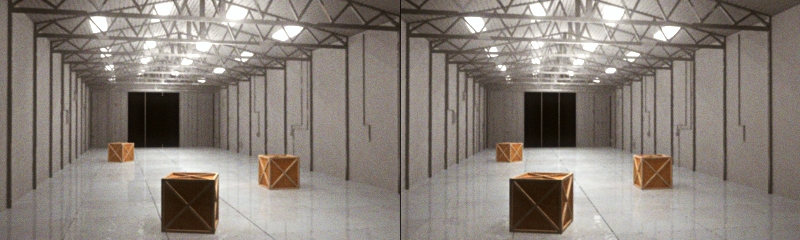
\includegraphics[width=13cm]{sbs.jpg}
 		\captionsetup{font={up, footnotesize}}
    	\caption{Stereogram typu side by side\cite{sidebyside}.}
 		\label{rys1}
\end{figure}

\subsubsection{Stereogramy typu single-image} 
Stereogramy typu single-image, inaczej nazywane autostereogramy, to zbiór punktów, które wydają się tworzyć trójwymiarową scenę, gdy są skośnie oglądane z bliska. Do osiągnięcia efektu stereoskopowego za pośrednictwem takich obrazów nie są potrzebne żadne urządzenia.

Przy długim wpatrywaniu się w specjalnie stworzony obraz powstaje wrażenie trójwymiarowości. Czasem autostereogramy mogą wyglądać jak zniekształcone lub losowo umieszczone kolorowe plamy. Taki wygląd w rzeczywistości nie jest przypadkowy, ponieważ poprzez użycie powtarzalnego wzoru są ukrywane obiekty trójwymiarowe \cite{stereoscopythesis}.

Gdy się patrzy na autostereogram, mózg początkowo widzi powtarzające się wzory dwuwymiarowe przez obojga oczu. Dzieje się tak dlatego, że mózg przede wszytskim skupia się na samym obrazie jako całości. Po jakimś czasie skupienia się na wzorze umieszczonym na obrazku oczy zaczynają patrzeć na niego pod nieco innym kątem. W tym momencie zaczyna działać stereoskopowy odbiór rzeczywistości i mózg jest w stanie skonstruować obraz trójwymiarowy \cite{autostereogramInfo}. Rysunek \ref{rys26} jest przykładem autostereogramu, gdzie pod powtarzającym się wzrorem można zobaczyć ośmiornicę.

\begin{figure}[H]
		\centering
 		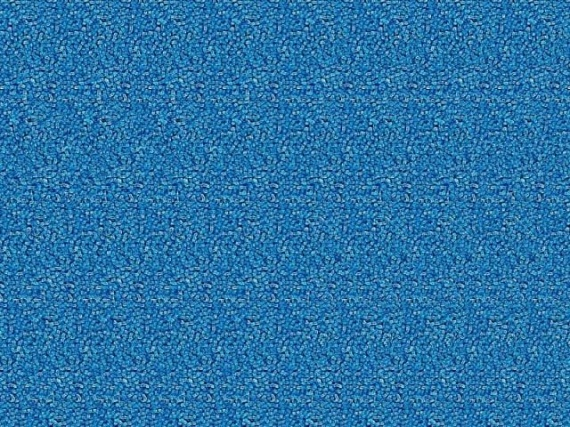
\includegraphics[width=9.0cm]{68.jpg}
 		\captionsetup{font={up, footnotesize}}
    	\caption{Autostereogram\cite{autostereogram}.}
 		\label{rys26}
\end{figure}

\subsubsection{Stereoskopia pasywna} 
Do tworzenia iluzji obrazów trójwymiarowych w tej technice są wykorzystywane specjalnie spolaryzowane okulary, które ograniczają światło docierające do każdego oka. W celu przedstawienia widoku stereoskopowego dwa obrazy są wyświetlane na tym samym ekranie z użyciem różnych filtrów polaryzacji. Istnieją 2 rodzaje filtrów: liniowe oraz kołowe.

W przypadku liniowej polaryzacji pole elektryczne światła jest skierowane pionowo bądź poziomo. Odbiorca zakłada odpowiednio dopasowane okulary, w których każda soczewka przepuszcza światło o innym kierunku polaryzacji. W ten sposób oczy obserwują różniące się obrazy. Minimalne pochylenie okularów może spowodować niezgodność polaryzacji światła a soczewek. Niepożądany efekt można wyeliminować, korzystając z filtrów kołowych prawo- lub lewoskrętnych. Ruch ten pozostaje niezmienny, nawet jeśli okulary są dowolnie pochylone\cite{russianpage}. Działanie polaryzacji kołowej prawoskrętnej zilustrowano na rysunku \ref{rys3}. 

\begin{figure}[H]
		\centering
 		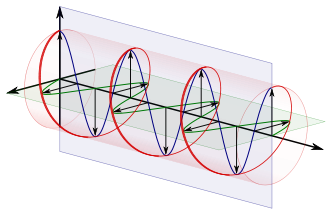
\includegraphics[width=7.0cm]{circular.png}
 		\captionsetup{font={up, footnotesize}}
    	\caption{Polaryzacja kołowa prawoskrętna \cite{polarization}.}
 		\label{rys3}
\end{figure}

Niewątpliwą zaletą stereoskopii spolaryzowanej jest to, że wiele osób może oglądać obrazy stereoskopowe w tym samym czasie. Wadą tego rozwiązania jest koszt specjalnego ekranu do wyświetlania obrazów. Taki ekran musi posiadać srebrną warstwę, dzięki czemu nie zniekształca się polaryzacja obrazów przy jednoczesnym wyświetlaniu.

\subsubsection{Stereoskopia aktywna} 
Z użyciem techniki stereoskopii aktywnej możliwość oglądania obrazów stereoskopowych pojawia się dzięki ciekłokrystalicznym okularom migawkowym. Szkło, które tworzy soczewki okularów, zawiera ciekłe kryształy oraz filtr polaryzacyjny. Stosując napięcie, można zmienić kolor soczewki na czarny, co bezpośrednio wiąże się z blokowaniem widoku dla jednego oka. Dzięki przykrywaniu widoku z dużą częstotliwością każdemu oku są przedstawiane obrazy z różną perspektywą \cite{active3d}. Częstotliwość migotania okularów jest zsynchronizowana z aktualnym źródłem wyświetlania, żeby stale dostarczać prawidłowej perspektywy dla oczu. Jeśli prędkość aktualizacji soczewek w okularach nie jest wystarczająco wysoka, to może nastąpić zauważalne zniekształcenie obrazu końcowego. Przykładem takiego zniekształcenia może posłużyć część obrazu ze złą perspektywą, przeznaczona innemu oku.

\subsubsection{Techniki anaglifowe}
Do generowania stereogramu anaglifowego potrzebne są 2 obrazy z delikatnie różniącą się perspektywą dla każdego oka. Każdy obraz jest wykonany w innym kolorze. Najbardziej popularną kombinacją jest obraz w kolorze czerwonym dla lewego oka i obraz wykonany w przy połączeniu zielonego i niebieskiego (otrzymany kolor nazywa się cyan) odpowiednio dla prawego oka. Obrazy umieszcza się jeden na drugim. Efekt stereoskopowego widoku jest osiągany przy użyciu okularów z poprawnymi kolorowymi filtrami (podobnie jak obrazy: czerwony dla lewego oka, cyan dla prawego). Niestety przy użyciu tej techniki nigdy nie zostanie stworzony pełnokolorowy obraz, gdyż barwy widziane przez każde oko są ograniczane \cite{anaglif}. 

Istnieją także filtry o innych kolorach, zachowujące główną zasadę anaglifów: przedstawienie innych obrazów każdemu oku poprzez ograniczenie pewnych barw.

Jest to jedna z najstarszych technik stereoskopowych, używana początkowo do tworzenia filmów 3D (pozbawionych barw) \cite{anaglifInfo}. Natomiast obecnie jednym z najciekawszych zastosowań techniki anaglifowej jest inicjatywa NASA, pokazująca powierzchnię Księżyca w postaci obrazów anaglifowych, rysunek \ref{rys4}.

\begin{figure}[H]
		\centering
 		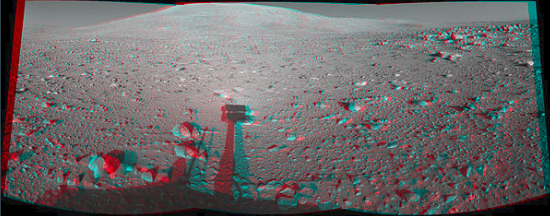
\includegraphics[width=12.5cm]{NASA.png}
 		\captionsetup{font={up, footnotesize}}
    	\caption{Teren Księżyca \cite{anaglif}.}
 		\label{rys4}
\end{figure}

\subsubsection{Wizualizacja wielopasmowa}
Nowa technika wyświetlania obrazów stereoskopowych, znana również pod tytułem INFITEC (ang. Interference filter technique, czyli technika filtrowania interferencyjnego). Główna jej idea jest podobna do stereoskopii anaglifowej: pokazanie dwóch obrazów z różniącą się perspektywą, które są wykonane w różnych kolorach. Jednak do osiągnięcia efektu stereoskopowego za pośrednictwem wizualizacji wielopasmowych jest wykorzystany fakt, że widmo światła widzialnego można podzielić na fale o różnej długości, używając do tego filtrów optycznych \cite{infitec}.

Światło widzialne jest podzielone na 6 części, po 2 na każdy z podstawowych kolorów: czerwony, zielony oraz niebieski. W ten sposób jednemu oku są przeznaczone 3 części (dla każdego podstawowego koloru po jednej). Ten podział umożliwia dostarczenie lekko różniących się barw do każdego oka z osobna. Wykorzystując niewystarczającą wrażliwość mózgu na tak niedużą różnicę, technika wizualizacji wielopasmowej stwarza obrazy pełnokolorowe. 

\subsubsection{Porównanie technik stereoskopowych}
Tabela \ref{tab11} przedstawia główne kryteria porównania technik stereoskopowych. Przede wszystkim zwracano uwagę na konieczność użycia  specjalistycznego sprzętu 3D do wyświetlenia obrazów oraz na jakość efektu. 

\begin{table}[H]
\caption{Porównanie technik stereoskopowych.}
\centering
\footnotesize
\label{tab11}
\begin{tabular}{!{\color{sapphire}\vrule width 1pt}m{0.146\textwidth}!{\color{black}\vrule width 1pt}m{0.146\textwidth}!{\color{black}\vrule width 1pt}m{0.146\textwidth}!{\color{black}\vrule width 1pt}m{0.126\textwidth}!{\color{black}\vrule width 1pt}m{0.136\textwidth}!{\color{black}\vrule width 1pt}m{0.126\textwidth}!{\color{sapphire}\vrule width 1pt}}
	\arrayrulecolor{sapphire}\hline
	\Centering\bfseries Nazwa technologii &
	\Centering\bfseries Kolory &
	\Centering\bfseries Rozdzielczość &
	\Centering\bfseries Specjalny monitor &
	\Centering\bfseries Liczba widzów &
	\Centering\bfseries Koszt \\
	\hline
	\arrayrulecolor{black}
	Side by side & Obraz pełnokolorowy & Wysoka & Niekonieczny & Ograniczona & Średni \\ 
	\hline
	Single image & Całkowity brak kolorów & Średnia & Nie & Ograniczona & Niski \\ 
	\hline
	Stereoskopia pasywna & Obraz pełnokolorowy & Wysoka & Tak & Duża & Średni \\ 
	\hline
	Stereoskopia aktywna & Obraz pełnokolorowy & Wysoka & Tak & Ograniczona & Wysoki \\ 
	\hline
	Anaglify & Całkowity brak kolorów & Średnia & Nie & Duża & Bardzo niski \\ 
	\hline
	Wizualizacje wielopasmowe & Obraz pełnokolorowy & Wysoka & Nie & Ograniczona & Bardzo wysoki \\ 
	\arrayrulecolor{sapphire}\hline
\end{tabular}
\end{table}

Po przeanalizowaniu opisanych technik zostały wybrane 2 do głębszego przestudiowania: technika stereoskopii pasywnej oraz technika stereoskopii aktywnej. Obie techniki wyróżniają się na tle innych, gdyż mają najlepszy stosunek jakości obserwowanych obrazów do kosztu ich wytwarzania. Zostaną one użyte w oprogramowaniu końcowym.


\subsection{Nvidia 3D Vision --- implementacja stereoskopii aktywnej}
Nvidia --- amerykańska firma komputerowa, która obecnie jest jednym z największych na świecie producentów procesorów graficznych (GPU, ang. Graphics Processing Unit, wysokowydajny procesor graficzny, potocznie nazywany kartą graficzną), który potrafi tworzyć realistyczne interaktywne obrazy na stacjach roboczych, komputerach osobistych, konsolach do gier i urządzeniach mobilnych \cite{NvidiaInfo}.

Rozwiązania technologiczne tej firmy cieszą się popytem na całym świecie. Jedną z najbardziej znanych marek procesorów graficznych jest GeForce (ang. Geometry Force, siła geometrii), zaprojektowany przez Nvidię, początkowo przeznaczony wyłącznie dla graczy. Obecnie architektura GeForce jest rozwijana w kierunku procesora graficznego ogólnego przeznaczenia (ang. GPGPU, general-purpose graphics processor unit). Ma to rozszerzyć funkcjonalność GPU poza tradycyjną rasteryzację grafiki 3D, przekształcając go w bardzo wydajne urządzenie komputerowe, które potrafi wykonywać kod dowolnego oprogramowania w taki sam sposób, jak robi to zwykły procesor \cite{GeForce}. 

Dla bezproblemowego korzystania z technologii postawiono następujące wymagania systemowe: 

\begin{itemize}
\itemi system operacyjny Microsoft Windows w wersjach Vista 32(64) bity lub 7 32(64) bity (nowsze wersje także są akceptowalne);
\itemi procesor  Intel Core2 Duo lub AMD Athlon X2 (ewentualnie nowsze wersje);
\itemi co najmniej 1GB pamięci RAM, aczkolwiek zaleca się 2GB;
\itemi minimum 100 MB wolnej pamięci na dysku;
\end{itemize}

\subsubsection{Szegółowy opis zestawu 3D Vision}
3D Vision (wcześniej GeForce 3D Vision) to zestaw dla widzenia stereoskopowego, również opracowany przez firmę Nvidia. Zestaw 3D Vision jest skierowany głównie do graczy i twórców gier komputerowych, ponieważ wyróżniona została jakość obrazów i duża prędkość ich przetwarzania. Sterownik Nvidia 3D Vision jest w stanie zinterpretować dowolną grę na wyświetlaczach o wystarczająco dużej szybkości odświeżania \cite{NvidiaInfo}. 

\begin{figure}[H]
		\centering
 		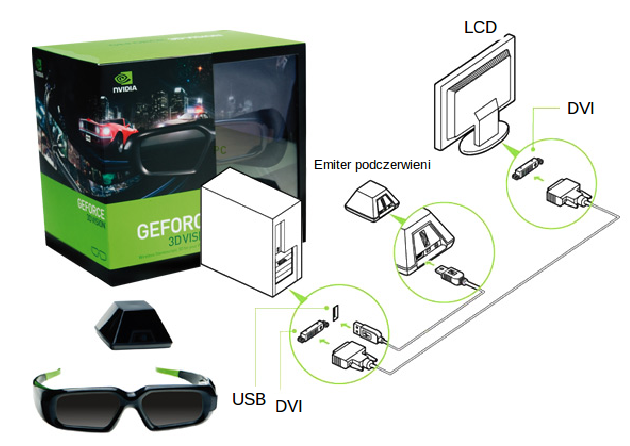
\includegraphics[width=7cm]{3dVision.png}
 		\captionsetup{font={up, footnotesize}}
    	\caption{3D Vision wraz z diagramem poprawnego ustawienia \cite{3dVisionPic}.}
 		\label{rys29}
\end{figure}

Podstawowy zestaw 3D Vision według oficjalnej strony internetowej \cite{3dVisionInfo} składa się z: 
\begin{itemize}
\itemi aktywnych okularów migawkowych, zapewniających dwukrotnie lepszą rozdzielczość dla każdego oka i szerszy kąt widzenia w porównaniu do okularów pasywnych;
\itemi emitera podczerwieni wysokiej mocy, przesyłającego dane bezpośrednio do aktywnych okularów migawkowych;
\itemi monitora z częstotliwością odświeżania co najmniej 120 Hz, pozwalającego uzyskać krystalicznie czyste, pozbawione migotania stereoskopowe obrazy 3D;
\itemi bezpłatnej przeglądarki 3D Vision, pozwalającej użytkownikom robić zrzuty ekranu w grze i wyświetlać je w 3D;
\itemi zaawansowanego oprogramowania Nvidia, automatycznie konwertującego ponad 300 gier do wyświetlenia w technologii aktywnej stereoskopii. 
\end{itemize}

\subsubsection{Sposób działania sterownika}
Wewnątrz sterownika każda scena 3D jest tworzona dwukrotnie --- raz dla lewego oka i raz dla prawego. Sterownik jest w stanie zmodyfikować typowe moduły cieniujące gier czasie rzeczywistym, żeby móc generować poprawne obrazy w trakcie wykonywania programu. Opcje dostępne użytkownikom pozwalają na zostosowanie ustawień indywidualnych, takich jak odległość między oczami czy wartość głębi obrazu. Natomiast twórcom oprogramowania umożliwiono bezpośrednie sterowanie aspektami stereo \cite{3dVisionInfo}.

W celu umożliwienia jak największej liczbie programistów stworzenie obrazów stereoskopowych dla wyświetlenia aktywnego jest rozwijana technologia Nvidia 3D Vision Automatic. W tej chwili ta technika nie jest jeszcze dostępna dla OpenGL, lecz została opublikowana działająca wersja dla OpenGL ES pod systemem Android 3.2 (lub nowszej wersji) dla urządzeń z procesorem Tegra 3 (lub nowszym).

\subsection{Biblioteka OpenGL}
Biblioteka OpenGL jest potężnym standardem stanowiącym niejako pomost między programistą a sprzętem komputerowym. Procedury OpenGL umożliwiają renderowanie obiektów o różnych poziomach skomplikowania, zaczynając od prostego punktu geometrycznego, linii lub wypełnionego wielokąta do utworzenia najbardziej złożonej, zakrzywionej powierzchni, oświetlonej i odwzorowanej teksturą. OpenGL pozwala programistom na dostęp do prymitywów geometrycznych i obrazowych, przekształcenia modelu, oświetlenia i teksturowania, antyaliasingu i wielu innych funkcji. 

Biblioteka OpenGL jest powszechnie dostępna na wszystkich jednostkach od komputerów o niskich kosztach, po wysokiej klasy stacjach roboczych i superkomputerach \cite{openglofficial}. Cały proces transformacji jest zarządzany poprzez potok graficzny OpenGL. Taki ciąg jest podzielony na poszczególne kroki, gdzie na wejściu są wymagane dane wyjściowe poprzedniego kroku. Każda z operacji jest dobrze sprecyzowana, gdyż mają one konkretną funkcję. 

\subsubsection{Moduły cieniujące}
Poprzez zgrupowanie poszczególnych kroków w potoku przetwarzania OpenGL powstaje schemat uproszczony. Został on przedstawiony na rysunku \ref{rys8}.

Dla każdego kroku przetwarzania, w celu konfiguracji obliczeń, są uruchamiane nieduże programy w procesorze graficznym --- moduły cieniujące. Te programy są pisane w języku w dużym stopniu podobnym do C --- GLSL (ang. OpenGL Shading Language, język cieniowania OpenGL). GLSL jest dostosowany do wykorzystania w grafice, ponieważ zawiera przydatne funkcje skierowane na manipulacje wektorami i macierzami. 

Moduły cieniujące zawsze zaczynają się od deklaracji wersji, następnie deklarowane są listy zmiennych wejściowych i wyjściowych, uniformy oraz ich główne funkcje. Uniform --- sposób przekazywania parametrów do modułów cieniujących \cite{slownik}. 

\begin{figure}[H]
		\centering
 		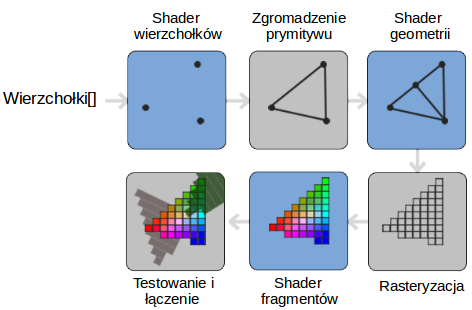
\includegraphics[width=11.5cm]{pipeline.png}
 		\captionsetup{font={up, footnotesize}}
    	\caption{Skrócony schemat potoku przetwarzania \cite{opengltutorial}.}
 		\label{rys8}
\end{figure}
\begin{itemize}

\itemi Moduł cieniujący wierzchołków (ang. vertex shader) jest programem, który realizuje pierwszy i zarazem fundamentalny etap potoku ---przetwarzanie danych związanych z wierzchołkami, w tym różnych atrybutów przekazanych wraz z położeniem wierzchołka. Na tym etapie między innymi obliczane są współrzędne wierzchołka na podstawie jego położenia porządkowego i macierzy przekształceń \cite{slownik}.
\itemi Montaż prymitywu (ang. primitive assembly). Jest to krok, który za dane wejściowe przyjmuje wszystkie wierzchołki (lub jeden, jeśli wybrana jest flaga GL\_POINTS ) z modułu cieniującego wierzchołków. Na tym etapie przetwarzania są kształtowane prymitywy --- wszystkie wierzchołki są grupowane do zadanego kształtu \cite{opengltutorial}.
\itemi Moduł cieniujący geometrii (ang. geometry shader). Program przyjmuje jako argumenty wejściowe kolekcję wierzchołków, które tworzą zadany kształt. W tym module również istnieje możliwość generowania innych kształtów poprzez emitowanie nowych wierzchołków, tworzących nowe (lub inne) prymitywy \cite{slownik}.
\itemi Rasteryzacja. W tym kroku uzyskane wcześniej prymitywy są mapowane na odpowiadające im piksele na ekranie. W wyniku powstają fragmenty do przetwarzania w kolejnym etapie, lecz zanim zostanie uruchomiony moduł cieniujący fragmentów, jest wykonywane przycinanie. Przycinanie pozwala odrzucić wszystkie fragmenty, które są poza zasięgiem obserwatora. Ów krok pozwala znacznie zwiększyć wydajność całego potoku. Fragment w OpenGL zawiera wszystkie niezbędne dane do wyświetlenia pojedynczego piksela \cite{slownik}.
\itemi Moduł cieniujący fragmentów. Głównym celem tego programu jest obliczenie końcowego koloru piksela i jest to zazwyczaj etap, na którym występują wszystkie zaawansowane efekty OpenGL. Z reguły moduł posiada wszystkie dane o scenie 3D (takie jak światła, cienie, kolor światła itp.), które są niezbędne dla określenia ostatecznej wartości koloru piksela \cite{slownik}.
\itemi Moduł cieniujący obliczeń (ang. compute shader) jest krokiem opcjonalnym, dostępnym w najnowszych wersjach OpenGL. Ten moduł cieniujący działa na zupełnie osobnym etapie GPU niż reszta potoku przetwarzania. Pozwala on aplikacji na korzystanie z mocy procesora graficznego do zadań ogólnych, które w większym lub mniejszym stopniu są powiązane z grafiką. Moduł cieniujący obliczeń ma dostęp do tych samych zasobów, co inne moduły cieniujące, jednak ma on większą kontrolę nad przepływem aplikacji i wykonaniem jej zadań \cite{OGlOfficialGuide}.
\end{itemize}

OpenGL nie zapewnia żadnej funkcjonalności do opisywania modeli obiektów trójwymiarowych, jak również nie posiada operacji odczytu obrazów z plików (na przykład o rozszerzeniu JPEG). Zamiast tego ta biblioteka daje duże możliwości w zbudowaniu trójwymiarowych obiektów z małego zestawu prymitywów geometrycznych --- punktów, krzywych, trójkątów i łat.

\subsection{Formaty plików 3D}
W celu ponownego wykorzystania skonstruowanych modeli 3D i przesłania ich na różne platformy, tworzone są pliki graficzne. Niemal każda duża platforma opracowała własny format plików 3D, dlatego powstało ich tak wiele, dla różnych aplikacji. Obecnie w grafice komputerowej istnieje ponad 70 odmiennych formatów \cite{formatslist}. Są one wykorzystywane w różnych dziedzinach, zaczynając od druku 3D, gier komputerowych, aż po medycynę i nauki przyrodnicze.

Podstawowym celem formatu pliku 3D jest przechowywanie informacji o modelu w postaci tekstu lub danych binarnych. W szczególności musi on zawierać dane o geometrii modelu, jego wyglądzie, scenie oraz animacjach. Geometria modelu opisuje jego dokładny kształt, do wyglądu zalicza się kolory, tekstury, typy wykorzystanych materiałów. Dane o scenie opisują między innymi położenie światła, kamery i obiektów peryferyjnych.

U podstaw każdego oprogramowania graficznego znajduje się biblioteka niskiego poziomu, taka jak OpenGL czy Direct3D. Biblioteki niskiego poziomu faktycznie rysują modele 3D na ekranie. Narzędzia autorskie wspierają modelowanie, zapewniają użytkownikom wygodne metody tworzenia, przeglądania, modyfikowania i zapisywania stworzonych modeli. Często oprogramowanie autorskie zawiera w sobie również przeglądarkę 3D --- narzędzie graficzne, które odczytuje, analizuje i transformuje pliki 3D do wewnętrznych formatów, a następnie wyświetla użytkownikowi.

W dalszej części tej pracy dyplomowej są przedstawione krótkie opisy najczęściej używanych formatów plików 3D. Na koniec tego podrozdziału jest umieszczone porównane formatów plików pod względem rozmaitości informacji, które one są w stanie przechowywać. Ma to pomóc w wyborze formatu pliku do przechowywania danych o modelu detektora ALICE.

\subsubsection{COLLADA}
COLLADA (ang. COLLAborative Design Activity) obsługuje wszystkie funkcje potrzebne współczesnym aplikacjom interaktywnym do tworzenia modeli 3D i pełnego przechowywania danych dotyczących tych modeli. Format został opracowany przez pracowników firmy Sony Computer Entertainment, ale od dłuższego czasu jest on własnością spółki Khronos Group, która obecnie współdzieli prawa autorskie z Sony. 

Stworzenie COLLADY miało na celu udostępnienie narzędzia, które byłoby przydatne dla jak najszerszego grona odbiorców. W tej chwili dziesiątki komercyjnych studiów gier i silników gier komputerowych przyjęły ten standard. Specyfikacja COLLADA jest upubliczniona na stronie internetowej zespołu technicznego Khronos Group \cite{colladaInfo}, który zajmuje się dalszym rozwojem formatu.

COLLADA to format pliku 3D z rozszerzeniem .DAE, powszechnie jest używany do modelowania w grach komputerowych i filmografii. W całości opiera się na strukturalizowaną reprezentację w XML. Przechowuje wszystkie dane dotyczące modelu 3D, jest to jeden z niewielu formatów wspierających kinematykę i informacje o cieniowaniu \cite{colladaInfo}.

Struktura formatu zaczyna się w korzeniu zwanym COLLADA, który zawiera elementy mianowane bibliotekami i sceną. Element scena mieści w sobie odnośnik do rzeczywistego początku hierarchii sceny. Natomiast każdy element "biblioteka"\ składa się ze specjalnych zestawów danych dokładnie opisujących model: informacje o siatce (library\_geometries), obrazie (library\_images) itd. Taki podział jest bardzo wygodny pod względem odwoływania się do konkretnych sekcji.

W ramach przykładu w tabeli \ref{tab16} umieszczono kawałek kodu źródłowego, opisującego pojedynczy węzeł struktury COLLADA. Ten węzeł gromadzi dane o sześcianie. Węzeł <mesh> (siatka) określa położenia wierzchołków, z których składa się kostka. W następnym węźle jest opisana kolejność łączenia wierzchołków siatki.
\begin{table}[H]
\caption{Kod źródłowy pliku .DAE. Przykład siatki sześcianu.}
\label{tab16}
\begin{lstlisting}[frame=single]  % Start your code-block
 <library_geometries>
 <geometry id="box" name="box">
 <mesh>
 <source id="box-Pos">
 <float_array id="box-Pos-array" count="24">
 -0.5 0.5 0.5
 ...
 </float_array>
 </source>
 <vertices id="box-Vtx">
 <input semantic="POSITION" source="#box-Pos"/>
 </vertices>
  <p>0 4 2 4 3 4 1 4</p>
 ...
 </mesh>
 </geometry>
 </library_geometries>
\end{lstlisting}
\end{table}

\subsubsection{STL}
STL (ang. STereoLithography, stereolitografia) jest jednym z najważniejszych formatów plików w dziedzinie druku 3D, tworzenia prototypów oraz komputerowo wspieranej produkcji. Rozszerzenie odpowiadające temu formatowi to .STL. Są dostępne oba rodzaje reprezentacji: tekstowy i binarny, przy czym binarny jest częściej wykorzystywany ze względu na mniejszy rozmiar plików. 

W STL są pominięte takie dane jak wygląd, scena czy animacje. Jedyne ważne informacje w tym formacie to geometria obiektów, która jest zapisywana w postaci przybliżonej siatki trójkątów. Dla każdego trójkąta są przechowywane 2 rodzaje danych:
\begin{itemize}
\itemi współrzędne wierzchołków;
\itemi współrzędne normalnej, przy tym wektor powinien wskazywać na zewnątrz w odniesieniu do modelu 3D.
\end{itemize}
\begin{figure}[H]
		\centering
 		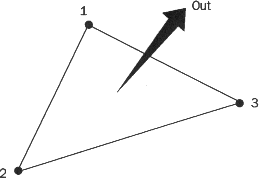
\includegraphics[width=5.0cm]{vertices-and-normal.png}
 		\captionsetup{font={up, footnotesize}}
    	\caption{Wierzchołki i normalna \cite{stlinfo}.}
 		\label{rys6}
\end{figure}
Dotychczas jest to najprostszy i najbardziej ścisły format przechowywania informacji o modelu 3D. Wadą STL jest brak przechowywania danych o kolorach, ze względu na dynamiczny rozwój technologii druku pełnokolorowego \cite{stlinfo}.

\subsubsection{OBJ}
OBJ jest jednym z najbardziej znanych i wykorzystywanych formatów plików 3D, obecnie nabiera szczególnej wagi w druku 3D. Ten format przechowuje informacje o modelu w postaci tekstu ASCII (rozszerzenie .OBJ) bądź pliku binarnego (rozszerzenie .MOD) \cite{objinfo}.
Format binarny jest zastrzeżony i nieudokumentowany, dlatego poniżej zostanie opisana tylko postać tekstowa formatu.

OBJ wspiera dane o prostych, wielokątach, krzywych oraz powierzchniach o różnych kształtach. Proste i wielokąty są opisywane poprzez wierzchołki, z których się składają. W przypadku krzywych oraz płaszczyzn kluczowymi są punkty kontrolne i inne niezbędne do opisu informacje, w zależności od typu krzywej. Ten format pliku 3D przybliża bądź oblicza dokładną siatkę bez drastycznego zwiększania rozmiaru pliku. Staje się to możliwe dzięki wykorzystaniu krzywych Beziera oraz metody NURBS (ang. Non-Uniform Rational Bezier Spline).

Format OBJ umożliwia również przechowywanie informacji o kolorach oraz teksturach modelu w towarzyszącym formacie MTL (ang. Material Template Library, Biblioteka Szablonów Materiałów). Plik .OBJ, po sparowaniu z odpowiednim plikiem .MTL, tworzy realistyczny wielokolorowy teksturowany model. Plik MTL jest zapisywany w postaci tekstu ASCII definiującego właściwości materiałów, odbijania światła itd. Dodatkowo MTL wspiera mapy tekstur, w tym przypadku każdy wierzchołek siatki modelu 3D jest przyporządkowywany do dwuwymiarowego obrazu \cite{mtlInfo}.

\subsubsection{3DS}
3DS to binarny format pliku początkowo wykorzystywany tylko w programie Autodesk 3D Studio. Plik binarny jest oparty o hierarchiczną strukturę "klocków"\ (ang. chunks), w której każdy fragment danych jest umieszczony w bloku z odpowiednim identyfikatorem. Pozwala to analizatorowi składni pominąć fragmenty, które nie są rozpoznawalne, oraz zapewnia możliwość rozszerzenia formatu \cite{3dsformat}.

3DS przechowuje tylko podstawowe informacje o geometrii, wyglądzie (kolory, tekstury i materiały), scenie oraz animacji. Gromadząc dane o scenie, zapisuje położenie kamer i świateł, z wyjątkiem informacji o kierunkowych źródłach światła. Do przybliżenia kształtu obiektu w formacie 3DS używa się siatki trójkątów, ale liczba wierzchołków i wielokątów nie może przekraczać 65536 ($2^{16}$).

Ten format jest obsługiwany praktycznie przez wszystkie pakiety oprogramowania 3D. Ze względu na to, że jednak 3DS zbiera tylko podstawowe informacje o modelu 3D, może on być uzupełniony o format MAX (obecnie zastąpiony formatem PRJ), który zawiera dodatkowe informacje specyficzne dla Autodesk 3DS Max, aby umożliwić całkowite zapisanie i załadowanie sceny.

\subsubsection{X3D}
Początkowo X3D nazywał się VRML (rozszerzenie pliku .WRL), z ang. Virtual Reality Modeling Language, czyli Język Modelowania Rzeczywistości Wirtualnej. Format został opracowany na potrzeby WWW (ang. World Wide Web), z czasem został zastąpiony przez X3D. Jest oparty o składnię XML.

X3D wykorzystuje siatkę wielokątów do zakodowania kształtu modelu, umożliwia przechowywanie wyglądu i danych, które wiążą się z tym parametrem. Na przeciągu ostatnich lat rozwoju tego formatu zostały dodane: kodowanie NURBS powierzchni geometrii, a także możliwość gromadzenia danych o scenie i animacjach \cite{formatsinfo}.

\subsubsection{Porównanie formatów plików}
Tabela \ref{tab1} przedstawia porównanie opisanych formatów plików 3D pod względem różnorodności przechowywanych danych.

Z tabeli wynika, że najwięcej informacji przechowują formaty COLLADA i X3D. Na potrzeby niniejszej pracy dyplomowej zostanie użyty format COLLADA.

Przede wszystkim dlatego, że pliki z rozszerzeniem .DAEsą łatwe zarówno do stworzenia, jak i do odczytania, ze względu na swoją strukturę. W dodatku są dostępne opracowane i przetestowane narzędzia do parsowania plików w tym formacie.

\begin{savenotes}
\begin{table}[H]
\caption{Macierz funkcjonalności najpopularniejszych formatów plików 3D}
\centering
\footnotesize
\label{tab1}
\begin{tabular}{!{\color{sapphire}\vrule width 1pt}c!{\color{black}\vrule width 1pt}c!{\color{black}\vrule width 1pt}c!{\color{black}\vrule width 1pt}c!{\color{black}\vrule width 1pt}c!{\color{black}\vrule width 1pt}c!{\color{black}\vrule width 1pt}c!{\color{black}\vrule width 1pt}c!{\color{black}\vrule width 1pt}c!{\color{black}\vrule width 1pt}c!{\color{black}\vrule width 1pt}c!{\color{sapphire}\vrule width 1pt}}
\arrayrulecolor{sapphire}\hline
\multirow{2}{*}{\bfseries Format} &
\multicolumn{3}{c!{\color{black}\vrule width 1pt}}{\bfseries Geometria} &
\multicolumn{3}{c!{\color{black}\vrule width 1pt}}{\bfseries Wygląd} &
\multicolumn{3}{c!{\color{black}\vrule width 1pt}}{\bfseries Scena} &
\multirow{2}{*}{\bfseries Animacje}\\
\cline{2-10}
& Przybl.\footnote{Przybliżona siatka}&Dokł.\footnote{Dokładna siatka}&CSG\footnote{CSG (ang. constructive solid geometry, strukturalna geometria bryły) – technika definiowania nowych brył poprzez łączenie innych brył}& Kolor& Materiał&Tekstura&Kamera&Światło&Pozycje& \\
\hline
COLLADA & X & X & & X & X & X & X & X & X & X\\
\arrayrulecolor{black}
\hline
STL & X & & & & & & & & & \\
\hline
OBJ & X & X & & X & X & X & & & & \\
\hline
3DS & X & & & X & X & X & X & X & X & \\
\hline
X3D & X & X & X & X & X & X & X & X & X & X\\
\arrayrulecolor{sapphire}\hline
\end{tabular}
\end{table}
\end{savenotes}

\subsection{Biblioteki do czytania i pisania modeli 3D}
Niestety, graficzne biblioteki niskiego poziomu takie jak OpenGL czy DirectX nie zapewnią żadnego mechanizmu do ładowania, zapisywania lub manipulowania modelami 3D. Dlatego, powstała potrzeba stworzenia nowych bibliotek ułatwiających te czynności. 

\subsubsection{Assimp}
Assimp (ang. Open Asset Import Library, Biblioteka Importowania Zasobów) to przenośna biblioteka do importowania różnych dobrze znanych formatów modeli 3D w jednolity sposób. Najnowsza wersja potrafi nie tylko czytać, ale również i zapisywać pliki 3D, i dlatego nadaje się jako transformator modeli 3D do ogólnego zastosowania. Assimp jest napisana w języku C++, istnieje również API (ang. Application Programming Interface, Interfejs Programistyczny Aplikacji) w języku C, a także jest powiązana z innymi językami programowania, w tym C\#, .net, Python i D.

Assimp ładuje wszystkie formaty modeli wejściowych do jednej prostej struktury danych w celu dalszego przetwarzania. Podstawowy zestaw funkcji jest rozszerzany przez różne narzędzia do przetwarzania końcowego. Przykładem rozszerzenia mogą posłużyć często potrzebne operacje, takie jak obliczanie wektorów normalnych i stycznych \cite{assimp}.

\subsubsection{Lib3ds}
Lib3ds to darmowa alternatywa dla pakietu 3DS File Toolkit firmy Autodesk do zarządzania plikami 3DS. Ta biblioteka jest w całości napisana w języku C, wspierana przez takie platformy jak GNU, UNIX, Mac OS X, Microsoft Visual C++. Jest łatwo integrowalna z biblioteką OpenGL \cite{lib3dsofficial}.

Celem lib3ds jest uproszczenie tworzenia filtrów do czytania i pisania plików formatu 3DS. Ta biblioteka jest obsługiwana na różnych rodzajach procesorów (big oraz little endian), wspiera moduły wektorowe, kwaterniony, macierze, proste struktury danych, które można łatwo modyfikować, ocenę wszystkich danych animacji. Istnieje możliwość załadowania większości fragmentów 3DS, sekcje: materiały, kamera, światło, siatka i klucze \cite{lib3dsdirectory}.

\subsubsection{Rozwiązania alternatywne}
Na chwilę obecną absolutna większość programów korzystająca z OpenGL i modelów przechowywanych w innych plikach używa biblioteki Assimp do załadowania danych do aplikacji. Natomiast istnieje kilka alternatywnych rozwiązań, które są mniej popularne przez to, że są dopasowane tylko do wybranego formatu plików 3D.

Na przykład Tinyobjloader jest parserem plików w formacie .OBJ. Tinyobjloader jest stworzony w C++, nie wymaga instalowania dodatkowych bibliotek z wyjątkiem STL --- biblioteki do ładowania tekstur \cite{tinyobjloader}. Zaletą tego parsera jest prędkość sczytywania i dalszego przetwarzania danych. 

Rozwiązanie, które zostało przedstawione przez firmę Autodesk --- Autodesk FBX SDK, jest darmową, łatwą w obsłudze platformą programistyczną, napisaną w C++. Autodesk FBX SDK służy do tworzenia oprogramowania, które pomaga informatykom przenieść zawartość sceny do formatu FBX \cite{FBXSoftwareDevelopmentKit}.

\subsection{ALICE}
Detektor ALICE został zaprojektowany tak, żeby w najbardziej kompletny sposób badać cząstki powstałe w kolizjach, które mają miejsce w środku akceleratora. Do zrealizowania założeń, używa się wielu warstw różnych detektorów, z których każda dostarcza inny rodzaj informacji o przebiegu zderzenia. Dane są gromadzone w sposób umożliwiający zrekonstruowanie i zbadanie ewolucji systemu cząstek w przestrzeni i czasie \cite{aliceofficial}.

\subsubsection{Eksperyment}
W ekstremalnych warunkach temperatury i (lub) gęstości materia hadronowa topi się w osoczu wolnych kwarków i gluonów --- tak zwanej plazmy kwarkowo-gluonowej (ang. quark–gluon plasma --- QGP). Aby stworzyć odpowiednie warunki w laboratorium, ciężkie jony (np. cząstki ołowiu) przyspiesza się do niemal prędkości światła, po czym jest powodowana kolizja. Kluczowym rozważaniem dotyczącym eksperymentu ALICE jest zdolność do badania chromodynamiki kwantowej (ang.  quantum chromodynamics --- QCD) i kwarków w tych ekstremalnych warunkach. Odbywa się to przy użyciu cząstek, utworzonych wewnątrz gorącej objętości podczas jej rozszerzania się i ochładzania. Cząstki te żyją wystarczająco długo, aby dotrzeć do wrażliwych warstw detektora zlokalizowanych wokół obszaru oddziaływania.

 Fizyka w ALICE polega na tym, żeby być w stanie zidentyfikować wszystkie cząstki (tj. określić, czy są to elektrony, fotony, piony itd.), czy też określić ich ładunek. Wiąże się to w większości z różnymi sposobami oddziaływania cząstek z materią \cite{aliceexperiment}.


\subsubsection{Ślady cząstek i detektory}

Zespół detektorów cylindrycznych (od wewnątrz na zewnątrz: ITS\footnote{The Inner Tracking System} Drift, ITS Strips, TPC\footnote{The ALICE Time Projection Chamber}, TRD\footnote{The ALICE Transition Radiation Detector}) mierzy w wielu punktach (ponad 100 tylko dla TPC) przejście każdej cząstki przenoszącej ładunek elektryczny tak, że trajektoria jest dokładnie znana. Detektory ALICE są osadzone w polu magnetycznym (wytwarzanym przez duży czerwony magnes), wyginając w ten sposób trajektorie naładowanych cząstek. Krzywizna śladów pozwala na obliczenie pędu badanych cząstek. ITS jest tak precyzyjny, że cząstki, które są generowane przez rozkład innych cząstek o bardzo krótkim czasie życia, można zidentyfikować, widząc, że nie pochodzą one z punktu, w którym nastąpiła interakcja ("wierzchołek"\ zderzenia) \cite{trackingparticles}.

\begin{figure}[H]
		\centering
 		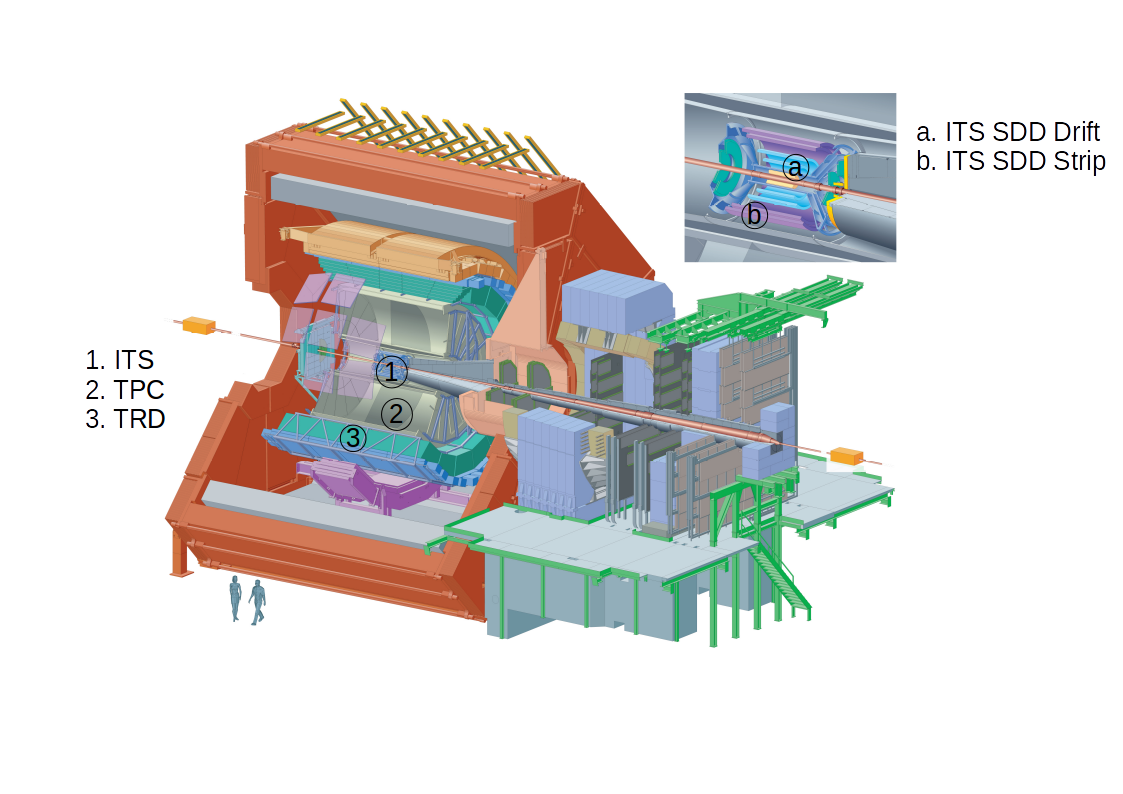
\includegraphics[width=16.0cm]{detector.png}
 		\captionsetup{font={up, footnotesize}}
    	\caption{Detektor ALICE \cite{aliceofficial}.}
 		\label{rys9}
\end{figure}
\subsubsection{Geometria detektora ALICE}
Budowanie, przeglądanie, śledzenie i wizualizacja geometrii detektora są dostępne w pakiecie geometrii ROOT --- TGeoManager. Kod tego oprogramowania nie zawiera żadnych ograniczeń związanych z fizyką cząstek, to znaczy, że nie jest on zależny od wyników symulacji zewnętrznych. Nie mniej jednak pakiet określa niektóre atrybuty, na które należy zwrócić uwagę: materiały, pole magnetyczne lub flagi stanu śladu cząstki. Ideą opracowania tego pakietu jest przechowywanie geometrii i jej użycie do różnych celów, na przykład do rekonstrukcji lub wizualizacji zderzeń cząstek \cite{TGeoManager}.

Rysowanie detektora w danym środowisku graficznym może przebiegać na wiele sposobów, w zależności od celu wybierane są funkcje i ich atrybuty. Istnieje możliwość narysowania detektora na różnych poziomach zagnieżdżenia się lub w różnych układach współrzędnych. Dla każdego przypadku jest zdefiniowana właściwa funkcja rysowania, której należy użyć. Rysunek \ref{rys27} jest wynikiem działania funkcji TGeoManager::SetVisLevel(Int\_t level), gdzie argument level przekazuje żądany poziom zagnieżdżenia się i, w tym przykładzie, wynosi 3.

\begin{figure}[H]
		\centering
 		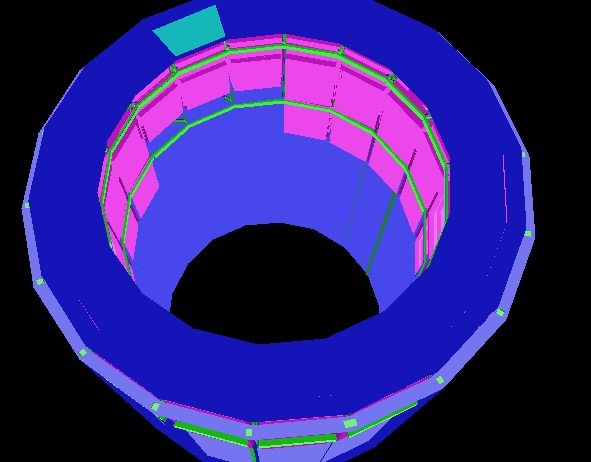
\includegraphics[width=10.0cm]{geometry.jpg}
 		\captionsetup{font={up, footnotesize}}
    	\caption{3. warstwa detektora ALICE \cite{TGeoManager}.}
 		\label{rys27}
\end{figure}

TGeoManager jest potężnym środowiskiem graficznym, posiadającym dziesiątki funkcji, opracowanych na potrzeby wizualizacji detektora. TGeoManager jest stworzony z użyciem biblioteki ROOT (napisanej w C++), która pośrednio korzysta z OpenGL.

Przez bardzo długi okres ROOT była rozwijana i dobudowywana, w wyniku tego powstała duża ilość kodu pomiędzy środowiskiem graficznym a OpenGL. W związku z powyższym, przejście do nowszych wersji oprogramowania leżącego u podstaw biblioteki ROOT stało się niezwykle skomplikowane. Pociągnęło to za sobą również problemy z użyciem już opracowanego modelu detektora ALICE w innych środowiskach.

\newpage
\section{Projekt oprogramowania}
Celem oprogramowania w niniejszej pracy dyplomowej jest wsparcie badania stereoskopowych wizualizacji oraz tworzenia realistycznych obrazów torów cząstek i detektora ALICE.

Założono, że program będzie wykonany w języku C++ z użyciem biblioteki OpenGL i bibliotek towarzyszących, takich jak na przykład GLFW czy GLM.

Na etapie analizy możliwych rozwiązań i technologii wykryto, że pobieranie danych o zderzeniach cząstek i o geometrii detektora bezpośrednio z CERN byłoby zbyt kosztowne czasowo, dlatego zostało zgłoszone zapotrzebowanie w plikach dostarczających te informacje. Dla przechowywania geometrii detektora wybrano format danych COLLADA, co wynikało z wcześniejszego przestudiowania dostępnych formatów i wybrania jednego, najbardziej dostosowanego do zadania. Dane o torach cząstek muszą być dostarczone w formacie JSON, gdyż jest to ustrukturyzowany format, pozwalający na łatwy zapis i odczyt informacji. W związku z powyższymi uwagami wiąże się wybór dodatkowych bibliotek wspierających program: JSONcpp, dla parsowania plików JSON, przechowujących dane o zderzeniach, i Assimp, dla wczytania modelu.

W części analitycznej zostały wybrane 2 techniki stereoskopowe dla dalszego przeanalizowania i wykorzystania w oprogramowaniu: stereoskopia pasywna i technika stereoskopii aktywnej. Obie metodyki wymagają specjalistycznego sprzętu. Tak w przypadku technologii pasywnej jest to: ekran 3D i specjalnie spolaryzowane okulary, natomiast stereoskopia aktywna wymaga kompletnego zestawu Nvidia 3D Vision. Cały sprzęt został udostępniony na cele badawcze w wydziałowym laboratorium grafiki komputerowej.

Żeby ułatwić korzystanie z programu, sterowanie widokiem będzie się sprowadzało do ruchów myszą i wciśnięcia określonych klawiszy. To ograniczenie w dużym stopniu redukuje niebezpieczeństwo wprowadzenia niepoprawnych danych, tym samym zmniejszając prawdopodobieństwo nieprzewidzianego zachowania programu.

Produktem końcowym jest program poprawnie tworzący i wyświetlający obrazy, zgodne z dostarczonymi danymi, który odpowiednio reaguje na działania użytkownika. Weryfikacja poprawności działania oprogramowania będzie polegała głównie na sprawdzeniu eksperymentalnym, czy stworzone obrazy rzeczywiście spełniają kryteria obrazów stereoskopowych.

\subsection{Wymagania funkcjonalne}
Zanim podjęto bezpośrednią pracę nad programem, sprecyzowano wymagania, jakie powinien spełniać końcowy produkt. Wymagania funkcjonalne wraz z opisami są spisane w tabeli \ref{tab2}. Podane zostały również priorytety każdego z wymagań (1 dla zadań najważniejszych) wyróżniające ważność wykonania zadania w całości.

\begin{table}[H]
\caption{Wymagania funkcjonalne.}
\centering
\footnotesize
\label{tab2}
\begin{tabular}{!{\color{sapphire}\vrule width 1pt}m{0.05\textwidth}!{\color{black}\vrule width 1pt}m{0.26\textwidth}!{\color{black}\vrule width 1pt}m{0.50\textwidth}!{\color{black}\vrule width 1pt}m{0.07\textwidth}!{\color{sapphire}\vrule width 1pt}}
\arrayrulecolor{sapphire}\hline
\Centering\bfseries Nr &
\Centering\bfseries Nazwa &
\Centering\bfseries Opis &
\Centering\bfseries Priorytet \\
\hline
\arrayrulecolor{black}
1 & Renderowanie torów cząstek & Program wyświetla ślady cząstek, odczytując kształt krzywych z położenia punktów kontrolnych z dostarczonego pliku JSON. & 1 \\
\hline
1.1 & Kolorowanie śladów & Tory są pokolorowane w zależności od masy cząstek. Dane są pobierane z dostarczonego pliku JSON. & 1 \\
\hline
2 & Renderowanie detektora & Program wyświetla detektor ALICE. Geometria detektora jest dostarczona w postaci pliku o rozszerzeniu .dae. Program odczytuje niezbędne dane z pliku, przetwarza je i wyświetla obraz na ekranie. & 1 \\
\hline
3 & Stworzenie efektu widzenia stereoskopowego & Program umożliwia oglądanie wyrenderowanych obrazów przy pomocy stereoskopii pasywnej. & 1 \\
\hline
4 & Stworzenie efektu aktywnego widzenia stereoskopowego & Program umożliwia oglądanie wyrenderowanych obrazów przy pomocy techniki aktywnego widzenia stereoskopowego. & 1 \\
\hline
5 & Możliwość interakcji z użytkownikiem & Program umożliwia użytkownikowi łatwe sterowanie położeniem oraz obrotami kamery. Funkcjonalność jest dostępna zarówno przy oglądaniu zwykłym, jak i stereoskopowym. & 2 \\
\arrayrulecolor{sapphire}\hline
\end{tabular}
\end{table}

\subsection{Wymagania niefunkcjonalne}
Wskazanie funkcji oprogramowania nie określa wszystkich cech istotnych dla użytkownika \cite{specyfikacja}. Wymagania niefunkcjonalne, które w danym zastosowaniu są ważne, zostały zdefiniowane i opisane w tabeli \ref{tab3}. Ze względu na badawczą specyfikę niniejszego programu zostały pominięte niektóre zalecane wymagania niefunkcjonalne. Tym zaś wymaganiom, które umieszczono poniżej, podobnie jak w przypadku wymagań funkcjonalnych zostały nadane priorytety.

\begin{table}[H]
\caption{Wymagania niefunkcjonalne.}
\centering
\footnotesize
\label{tab3}
\begin{tabular}{!{\color{sapphire}\vrule width 1pt}m{0.05\textwidth}!{\color{black}\vrule width 1pt}m{0.26\textwidth}!{\color{black}\vrule width 1pt}m{0.50\textwidth}!{\color{black}\vrule width 1pt}m{0.07\textwidth}!{\color{sapphire}\vrule width 1pt}}
\arrayrulecolor{sapphire}\hline
\Centering\bfseries Nr &
\Centering\bfseries Nazwa &
\Centering\bfseries Opis &
\Centering\bfseries Priorytet \\
\hline
\arrayrulecolor{black}
1 & Przenośność & Program działa bez błędów na różnych systemach operacyjnych (Windows, Linux). W systemie operacyjnym Linux dopuszczalny jest brak funkcjonalności aktywnego widoku stereoskopowego ze względu na zewnętrzne urządzenia. & 1 \\
\hline
2 & Zrozumiałość & Program jest łatwy w użyciu. & 1 \\
\hline
3 & Czytelność kodu źródłowego & Kod źródłowy programu jest napisany zgodnie z zasadami, wzorcami i najlepszymi praktykami branży. & 1\\
\hline
4 & Tolerowanie defektów & Przewidywalne zachowanie programu, pomimo pomyłek obsługi lub wprowadzenia błędnych danych. & 1 \\
\hline
5 & Przyjazność programu dla użytkownika & Program jest intuicyjny w obsłudze. & 2\\
\arrayrulecolor{sapphire}\hline
\end{tabular}
\end{table}

\newpage
\subsection{Przypadki użycia}
Wymagania użytkownika programu mogą być pokazane jak lista zadań, która może być wykonana z użyciem powstającego programu. W takim przypadku każde zadanie musi być opisane, z uwzględnieniem kolejności poszczególnych kroków, które by doprowadziły użytkownika do konkretnego miejsca w programie. Podsumowując, opis wymagań sprowadza się do opisu możliwych sposobów używania programu przez aktorów (użytkowników).

Graficzną reprezentacją modelu przypadków użycia jest rysunek \ref{rys34}.

\begin{figure}[H]
		\centering
 		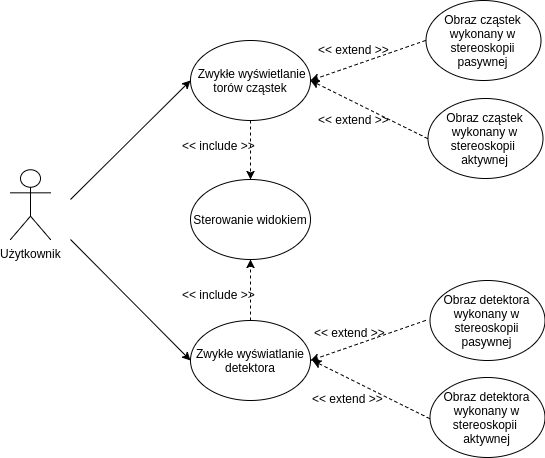
\includegraphics[width=14.0cm]{UseCase.png}
 		\captionsetup{font={up, footnotesize}}
    	\caption{Diagram przypadków użycia.}
 		\label{rys34}
\end{figure}

Aktorem w tym kontekście jest zwykły użytkownik programu. Przez to, że głównym celem tej oto pracy dyplomowej są wizualizacje, opis każdego przypadku użycia kończy się oglądaniem wygenerowanych scen oraz poruszaniem się w nich. Szczegółowe opisy przypadków użycia zostały umieszczone w tabeli \ref{tab4}.

\begin{table}[H]
\caption{Przypadki użycia programu}
\centering
\footnotesize
\label{tab4}
\begin{tabular}{!{\color{sapphire}\vrule width 1pt}m{0.05\textwidth}!{\color{black}\vrule width 1pt}m{0.16\textwidth}!{\color{black}\vrule width 1pt}m{0.50\textwidth}!{\color{black}\vrule width 1pt}m{0.17\textwidth}!{\color{sapphire}\vrule width 1pt}}
	\arrayrulecolor{sapphire}\hline
	\Centering\bfseries Nr &
	\Centering\bfseries Nazwa &
	\Centering\bfseries Opis &
	\Centering\bfseries Scenariusz alternatywny \\
	\hline
	\arrayrulecolor{black}
	FU1 & Wyświetlanie torów cząstek & 
	\begin{itemize}
	\itemi Użytkownik uruchamia program.
	\itemi Wybiera opcję zwykłego wyświetlania torów cząstek.
	\itemi Steruje kamerą przy pomocy klawiatury i myszy.
	\end{itemize} & Brak \\ 
	\hline
	FU2 & Wyświetlanie detektora & \begin{itemize}
	\itemi Użytkownik uruchamia program.
	\itemi Wybiera opcję zwykłego wyświetlania detektora.
	\itemi Steruje kamerą przy pomocy klawiatury i myszy.
	\end{itemize} & Brak \\ 
	\hline
	FU3 & Stereoskopowe wyświetlanie obrazów & \begin{itemize}
	\itemi Użytkownik uruchamia program.
	\itemi Wybiera opcję stereoskopowego wyświetlania detektora (lub torów cząstek).
	\itemi Przełącza ekran w tryb 3D oraz zakłada specjalne okulary.
	\itemi Steruje kamerą przy pomocy klawiatury i myszy.
	\end{itemize} & Brak \\ 
	\hline
	FU4 & Aktywne wyświetlanie obrazów stereoskopowych & \begin{itemize}
	\itemi Użytkownik uruchamia program.
	\itemi Wybiera opcję aktywnego wyświetlania obrazu stereoskopowego detektora (lub torów cząstek).
	\itemi Przełącza ekran w tryb aktywnego widzenia 3D oraz zakłada specjalne okulary.
	\itemi Steruje kamerą przy pomocy klawiatury i myszy.
	\end{itemize} & Brak \\ 
	\hline
	FU5 & Przełączenie widoków & \begin{itemize}
	\itemi Użytkownik uruchamia program.
	\itemi Wybiera opcję zwykłego wyświetlania torów cząstek.
	\itemi Wybiera opcję stereoskopowego wyświetlania detektora.
	\itemi Przełącza ekran w tryb 3D oraz zakłada specjalne okulary.
	\itemi Wybiera opcję zwykłego wyświetlania obrazu detektora. 
	\itemi Zdejmuje okulary 3D, przełącza ekran w tryb zwykłego wyświetlania.
	\itemi Steruje kamerą przy pomocy klawiatury i myszy.
	\end{itemize} & Brak \\ 
	\arrayrulecolor{sapphire}\hline
\end{tabular}
\end{table}

\subsection{Diagram klas}
Model przypadków użycia opisuje zachowanie programu z punktu widzenia przeciętnego użytkownika, nie określa on natomiast sposobu, w jaki
należy oprogramowanie stworzyć. Podstawowymi elementami programu napisanego w języku obiektowym są klasy. Mogą one być powiązane z innymi klasami programu na wiele różnych sposobów. Nieduży rozmiar programu pozwala na projektowanie architektury na poziomie klas.

Na tym etapie projektu diagram klas jest wciąż postrzegany tylko w perspektywie pojęciowej, gdzie nie podjęto jeszcze decyzji o dokładnym rozmieszczeniu w klasach metod implementujących przypadki użycia opisane w tabeli \ref{tab4}. Diagram na rysunku \ref{rys24} przedstawia wstępną wersję budowy klas w programie.

\begin{figure}[H]
\centering
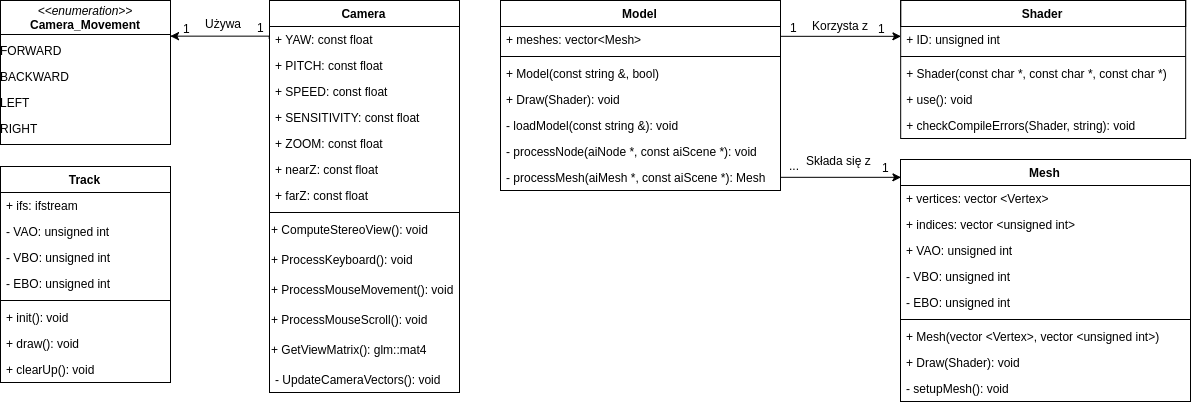
\includegraphics[width=13.0cm]{DiagramKlas.png}
\captionsetup{font={up, footnotesize}}
\caption{Diagram klas programu wizualizacji.}
\label{rys24}
\end{figure}

\subsubsection{Klasa Shader}
Pisanie, kompilowanie i zarządzanie modułami cieniującymi może być dość kłopotliwe. Dlatego postanowiono zebrać wszystkie metody dotyczące tych programów do wspólnej klasy Shader (moduł cieniujący). Ta klasa miałaby za zadanie odczytanie modułów z dysku, ich kompilację i łączenie, sprawdzałaby także błędy występujące w trakcie przetwarzania modułów cieniujących.

Zmienna ID jest unikatowym numerem każdego modułu cieniującego, wartość tej zmiennej określa się w momencie wywołania funkcji glCreateProgram(). Ta funkcja tworzy obiekt modułu cieniującego i zwraca referencję do jego numeru. Zmienna ID jest przydatna do odwołania się do pewnego modułu w trakcie działania programu.

Metoda use() zawierałaby w sobie wywołanie funkcji glUseProgram(ID). Funkcja glUseProgram instaluje obiekt modułu (podanego w argumencie wywołania) jako część bieżącego stanu renderowania.

\subsubsection{Klasa Camera}
Klasa Camera (kamera) odpowiadałaby za zmiany widoku przy interakcji z użytkownikiem. Zmiany widoku by zachodziły po wciśnięciu wybranych klawiszy, po poruszeniu myszą bądź tylko kółkiem myszy. Dodatkowo ta klasa obliczałaby widok stereoskopowy (computeStreoView), innymi słowy, tworzyłaby dwa obrazy z różniącą się perspektywą jako materiał stereoskopowy.

Wartość wyliczeniowa Camera\_Movement (ruch kamery) określałaby kierunek ruchu kamery w zależności od wciśniętego przycisku. Ułatwi to komunikację pomiędzy obsługą zdarzeń przychodzących z klawiatury a kamerą, owocując w odpowiednie przeliczania widoku w programie.

W klasie Camera również zostaną zdefiniowane takie zmienne globalne jak szybkość poruszania się kamery, wartości kątów obrotów czy wrażliwość kamery na ruchy myszy.

\subsubsection{Klasy Mesh i Model}
Klasy Mesh (siatka) i Model muszą zostać opracowane na potrzeby wczytania modelu z pliku o formacie COLLADA do programu. Konieczna będzie do zrealizowania zmiana struktur danych z biblioteki Assimp na konstrukcje obsługiwane przez OpenGL.

Obiekt typu Mesh będzie przechowywał odczytane informacje o poszczególnej siatce, natomiast obiekt typu Model będzie gromadził dane o modelu jako całości. Dla poprawnego wyświetlenia modelu detektora, wczytanego do obiektu typu Model, zaprojektowano połączenie Model-Shader.

\subsubsection{Klasa Track}
W klasie Track wczytywano by dane z pliku JSON. Funkcja init() aktualizowałaby bufory przesyłające informację prosto do karty graficznej, wypełniając je w dane, określając atrybuty odczytanych wierzchołków i określając kolejność wyświetlania wierzchołków. Ten krok przyspieszyłby generowanie sceny, nie wywierając negatywnych skutków na obrazach, przedstawiających tory cząstek po kolizji w detektorze.

Funkcja draw() umożliwiałaby bezpośrednie rysowanie ścieżek cząstek. Po zaalokowaniu pamięci na potrzeby buforów przyda się również funkcja zwalniająca ten zasób. Do usunięcia buforów z pamięci została wyznaczona funkcja cleanUp().

\subsection{Technologie}
\subsubsection{Dodatkowe biblioteki graficzne}
Biblioteka ładująca OpenGL (ang. OpenGL Loading Library) wciąga wskaźniki do funkcji OpenGL w środowisku wykonawczym, rdzeniu i rozszerzeniach. Jest to wymagane, aby uzyskać dostęp do funkcji OpenGL w wersjach powyżej 1.1 na większości platform. Duża liczba bibliotek ładujących rozszerzenia zastępuje potrzebę włączenia gl.h. Zamiast tego udostępniają własny nagłówek, który musi zostać użyty. Większość bibliotek ładowania używa specjalnego generatora do skonstruowania kodu, który wciąga wskaźniki funkcji i zawarte nagłówki \cite{LoadingLibrary}.

GLAD --- biblioteka generująca kod do ładowania GL. Za pomocą GLAD można wygenerować nagłówki lub kod źródłowy dla dowolnej wersji OpenGL, od wersji 1.1 do 4.6. Można również dołączyć dowolne rozszerzenia OpenGL.

GLFW --- biblioteka dla OpenGL rozwijana jako oprogramowanie otwarte (ang. open source). GLFW zapewnia łatwość w tworzeniu okien i kontekstów, w obsłudze danych i zdarzeń wejściowych. Biblioteka jest napisana w języku C, dzięki czemu jest wieloplatformowa.

Obsługę wielu okien, monitorów, ramp o wysokiej rozdzielczości DPI i gamma wymienia się jako jedną z największych zalet tej biblioteki. Oprócz tego, poprzez odpytywania obsługiwane są klawiatura, mysz, gamepad, okna zdarzeń oraz zarządzanie czasem, co jest bardzo wygodne w sterowaniu podczas tworzenia wizualizacji. W dodatku GLFW ma dostęp do rodzimych obiektów i opcji kompilacji dla specyficznych funkcji platform \cite{glfw}.

GLM (ang. OpenGL Mathematics, matematyka OpenGL) --- nagłówek do biblioteki matematycznej C++, opracowany dla oprogramowania graficznego opartego na specyfikacjach języka GLSL. GLM udostępnia klasy i funkcje zaprojektowane i zaimplementowane z użyciem tej samej konwencji nazewnictwa jak w GLSL. Biblioteka zapewnia rozszerzone możliwości: przekształcenia macierzy i kwaternionów, liczby losowe, szumy itd. GLM doskonale działa z OpenGL, nadaje do oprogramowania renderowania i rasteryzacji, przetwarzania obrazu, symulacji zjawisk fizycznych oraz wszelkich kontekstów rozwojowych, które wymagają prostej i wygodnej biblioteki matematycznej \cite{glm}.

\subsubsection{Glitter}
Założono, że projekt będzie łatwy w użyciu, lecz czasami instalowanie zależności może być bardzo frustrujące, szczególnie w środowiskach, w których brakuje zarządcy pakietów lub uprawnień administracyjnych, dlatego pierwsze skonfigurowanie programu może być dużym wyzwaniem. Dla zapewnienia przenośności oraz łatwości użycia opracowywanego programu skorzystano z gotowego prostego zestawu dla OpenGL pt. Glitter.

Glitter kompiluje i statycznie łączy wszystkie niezbędne biblioteki. Robi on to za pośrednictwem jednej zależności: cmake, która służy do generowania specyficznych dla platformy plików makefile lub plików projektu. Glitter łączy większość zależności potrzebnych do wdrożenia podstawowego mechanizmu renderującego \cite{glitter}, zawiera biblioteki:
\begin{itemize}
\itemi assimp
\itemi glfw
\itemi glm
\itemi glad
\end{itemize}

\subsubsection{JSONcpp}
JSONcpp --- biblioteka w języku C++ umożliwiająca manipulowanie wartościami JSON, w tym serializację i deserializację ciągów. Dzięki JSONcpp istenieje możliwość na odczytanie i zapisanie pliku formatu JSON, na dołączenie komentarzy w konwencji C++ do elementu podczas parsowania oraz przerobić plik JSON, zachowując oryginalne komentarze \cite{jsoncpp}.

Jednym ze sposobów integracji JSONcpp z projektem jest dołączenie plików z kodem źródłowym (pojedynczego pliku .cpp i dwóch plików .h) do projektu oraz ich kompilacja w taki sam sposób jak każdy inny plik źródłowy. Zapewnia to spójność flag kompilacji i kompatybilności, rozwiązuje problemy powstające podczas budowania bibliotek współdzielonych lub statycznych.

\newpage
\section{Część weryfikacyjna}
\subsection{Macierze modelu, widoku, projekcji}
Obraz wyświetlany na ekranie --- wierzchołki o konkretnych współrzędnych dwuwymiarowych przedstawiające scenę 3D, lecz początkowo scenę tworzy się w przestrzeni trójwymiarowej. Przejścia z jednego układu współrzędnych na inny są znacznie wygodniejsze przy użyciu macierzy transformacji: modelu, widoku oraz projekcji.

Lokalny układ współrzędnych to taki układ, w którym obiekt ma swój początek. Położenia wierzchołków obiektu są zmieniane względem początku układu lokalnego. Lokalne układy współrzędnych są przeliczane na współrzędne świata, dzięki temu obiekty są rozmieszczane w różnych miejscach sceny. W kolejnych krokach układ współrzędnych świata jest przekształcany na widok z perspektywy kamery. Po wprowadzeniu współrzędnych do widoku są one zmieniane na współrzędne rzutni. Decydującym faktem jest to, że współrzędne rzutni są przetwarzane w zakresie (-1.0; 1.0), określając jednoznacznie wierzchołki, które mają być wyświetlone na ekranie. Ostateczny obraz powstaje po przeliczeniu współrzędnych rzutni na współrzędne ekranu, które są następnie przesyłane do rasteryzatora. Opisane przejścia i transformacje macierzy są zilustrowane na rysunku \ref{rys11}.

\begin{figure}[H]
		\centering
 		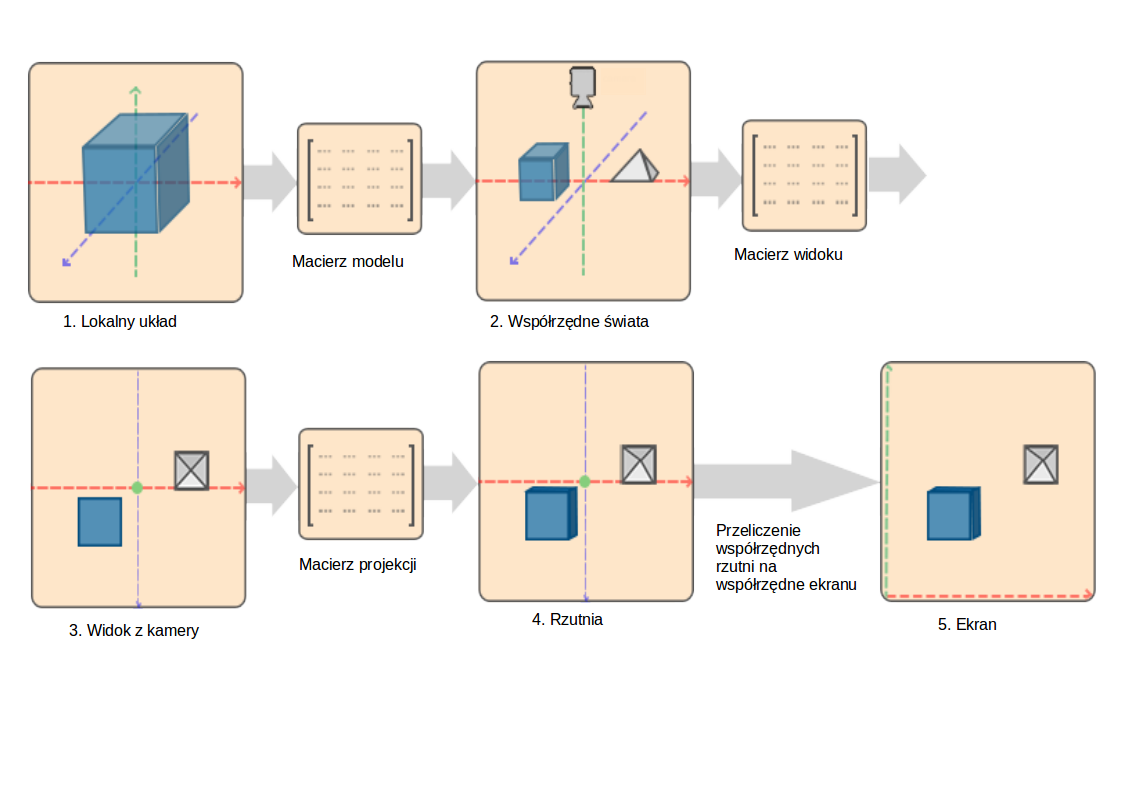
\includegraphics[width=12.0cm]{coordinate_systems.png}
 		\captionsetup{font={up, footnotesize}}
    	\caption{Przejścia z jednego układu współrzędnych na inny \cite{opengltutorial}.}
 		\label{rys11}
\end{figure}

W ramach rozwijanego programu przyjęto założenie, że wszystkie wierzchołki modelu są w lokalnym układzie współrzędnych obiektu. Natomiast macierz modelu reprezentuje  obiekt w układzie współrzędnych świata, ze względu na możliwość skalowania, obrotu czy translacji. Widok został przypisany do kamery. Macierz projekcji początkowo przypisywana jest do przestrzeni rzutni w zakresie (-1000; 1000) na każdej osi, lecz ostatecznie jest normalizowana do zakresu (-1.0; 1.0). Wszystkie wierzchołki umieszczone poza tym zakresem nie będą widoczne na ekranie.

\subsection{Kamera}
Jednym z wymagań funkcjonalnych było sterowanie kamerą w celu przesunięcia bądź przybliżenia widoku. Zgodnie z założeniem projektowym, w tym celu powstała klasa Camera (plik nagłówkowy Camera.h).

Podchodząc do rozwiązania tego zadania, przyjęto, że za pomocą macierzy widoku wszystkie współrzędne sceny będą przekształcane na współrzędne widoku względem położenia i kierunku patrzenia kamery. Stąd do zdefiniowania kamery niezbędne są:
\begin{itemize}
\itemi położenie kamery w scenie;
\itemi kierunek patrzenia kamery;
\itemi wektor skierowany w prawo od kamery;
\itemi wektor skierowany w górę od kamery.
\end{itemize}
W ten sposób został utworzony układ współrzędnych, gdzie położenie kamery jest punktem początkowym, a trzy pozostałe wektory to prostopadłe do siebie osie.

Funkcja glm::LookAt z biblioteki GLM przyjmuje jako argumenty położenie kamery, kierunek patrzenia oraz wektor skierowany w górę (tworzy z tego wektor skierowany w prawo od kamery), zwracając przy tym gotową macierz widoku. W głównym pliku programu została zdefiniowana funkcja processInput, która, używając biblioteki GLFW, zarządza danymi przychodzącymi z klawiatury. Dzięki tej funkcji łączone są określone klawisze z odpowiednimi zmianami położenia kamery, owocując przeliczeniem macierzy widoku.

Obroty kamery zostały zrealizowane przy użyciu macierzy obrotu i funkcji trygonometrycznych. Wartości odchylenia i nachylenia kamery, zgodnie z projektem, są pozyskiwane z ruchu myszy, gdzie poziomy ruch myszy wpływa na odchylenie, a pionowy odpowiednio na nachylenie. Zapamiętywana jest pozycja myszy w ostatniej klatce, a w aktualnej jest obliczana różnica wartości aktualnych i zapamiętanych. W zależności od wielkości obliczonych wartości porusza się kamera. Dla uniknięcia zbyt szybkich albo dużych odchyleń (lub nachyleń) zostały wprowadzone ograniczniki, zmniejszające zakres poruszania kamerą \cite{learnopengl}.

Również wprowadzono do programu obsługę przybliżenia. Zaimplementowano ten efekt, używając właściwości "pola widzenia"\ : jak pole widzenia staje się mniejsze, rzutowana przestrzeń sceny również się zmniejsza, dając iluzję powiększania obrazu. Do sterowania powiększaniem używa się kółka myszki.

\subsection{Rysowanie ścieżek cząstek}
W celu narysowania ścieżek cząstek niezbędne są wierzchołki składające się na nie. Zgodnie z założeniem początkowym są one odczytywane z pliku JSON. Współrzędne odczytanych wierzchołków są zapisywane do wspólnego wektora. Wraz ze ścieżkami są odczytywane masy cząstek, po których zostały ślady. Masa cząstki jest później używana do kolorowania toru.

\subsubsection{Odczytanie danych}
Proces odczytania danych ze specjalnie przygotowanego pliku JSON jest realizowany z użyciem biblioteki JSONcpp. W tabeli \ref{tab6} jest przedstawiony kawałek kodu źródłowego, który deserializuje dane JSON (Json::Reader readerTracks) i zapisuje odczytane wartości do wektora.

Json::Value reprezentuje wartość JSON, zmienna ifs przekazuje ścieżkę do pliku do strumienia wejściowego (ang. ifstream, strumień wejściowy do obsługi plików).

Otrzymany plik JSON ma następującą strukturę. W pojedynczych polach na początku pliku są przechowywane dane identyfikujące zderzenie: numer zderzenia, energię, system, w którym nastąpiła kolizja, czas oraz listę cząstek wytworzonych w wyniku zderzenia (fTracks). Każdy obiekt z listy fTracks gromadzi dane o cząstce, między innymi jej unikatowy numer, typ, masę (fMass), numer cząstki-rodzica oraz trzy listy współrzędnych toru tej cząstki. Każda lista przechowuje jedną składową współrzędnych wierzchołka kontrolnego: fPolyX, fPolyY oraz fPolyZ, odpowiednio (x; y; z).

Iterując najpierw po liście fTracks, a następnie po listach współrzędnych, sczytuje się dane o położeniu cząstki w przestrzeni. Kolor każdej ścieżki składa się z dwóch przeliczonych wartości masy oraz z wartości, która jest doliczana w module cieniującym fragmentów.

\begin{table}[H]
\caption{Kod źródłowy programu. Odczytanie danych z pliku JSON.}
\label{tab6}
\begin{lstlisting}[frame=single]  % Start your code-block

Json::Value objectTracks;
Json::Reader readerTracks;
readerTracks.parse(ifs,objectTracks);
for (Json::Value::iterator it = objectTracks["fTracks"].begin(); 
	it != objectTracks["fTracks"].end(); ++it){
 float color = (*it)["fMass"].asFloat();
 for (int i = 0; i < (*it)["fPolyX"].size(); i++){
  tracks.push_back((*it)["fPolyX"][i].asFloat());
  tracks.push_back((*it)["fPolyY"][i].asFloat());
  tracks.push_back((*it)["fPolyZ"][i].asFloat());
  tracks.push_back(color*0.9f);
  tracks.push_back(color*0.9f);
  indices.push_back(indicator);
  indicator++;}
 indices.push_back(GL_PRIMITIVE_RESTART_FIXED_INDEX);}}
\end{lstlisting}
\end{table}

Zdefiniowany w ten sposób wektor wierzchołków jest wysyłany na wejście modułu cieniującego wierzchołków dla dalszego przetwarzania. Odbywa się to poprzez zaalokowanie pamięci w procesorze graficznym, skonfigurowanie sposobu interpretowania tej pamięci przez OpenGL oraz określenie sposobu wysyłania danych do karty graficznej. Zatem moduł cieniujący wierzchołków przetwarza tylko taką liczbę punktów, jaka została zdefiniowana w pamięci.

\subsubsection{Definiowanie buforów}
Moduł cieniujący wierzchołków pozwala na określenie dowolnych danych wejściowych w postaci atrybutów wierzchołków. Oznacza to, że poszczególne części danych wejściowych są ręcznie przypisywane do atrybutów wierzchołka. W takim przypadku potrzebne jest określenie, w jaki sposób OpenGL będzie interpretować dane przed renderowaniem. Założono, że:
\begin{itemize}
\itemi dane pozycji są przechowywane jako 32-bitowe (4 bajty) wartości zmiennoprzecinkowe;
\itemi każda pozycja składa się z 5 wartości: 3 współrzędnych położenia i 2 pozycji koloru;
\itemi nie ma pustych miejsc w tablicy, wszystkie wartości są obok siebie;
\itemi pierwsza wartość jest początkiem bufora.
\end{itemize}
Używając funkcji glEnableVertexAttribArray, określono, w jaki sposób dane wierzchołków będą interpretowane. Przykład implementacji powyższych założeń jest przedstawiony w tabeli \ref{tab7}.

\begin{table}[H]
\caption{Kod źródłowy programu. Przekazanie danych do VAO, VBO i EBO.}
\label{tab7}
\begin{lstlisting}[frame=single]  % Start your code-block

glGenVertexArrays(1, &VAO);
glGenBuffers(1, &VBO);
glGenBuffers(1, &EBO);
glBindVertexArray(VAO);
glBindBuffer(GL_ARRAY_BUFFER, VBO);
glBufferData(GL_ARRAY_BUFFER, tracks.size() * sizeof(GLfloat),
  &tracks[0], GL_STATIC_DRAW);
glBindBuffer(GL_ELEMENT_ARRAY_BUFFER, EBO);
glBufferData(GL_ELEMENT_ARRAY_BUFFER, indices.size() * sizeof(GLuint),
  &indices[0], GL_STATIC_DRAW);
glVertexAttribPointer(0, 3, GL_FLOAT, GL_FALSE, 5 * sizeof(float),
  (void*)0);
glEnableVertexAttribArray(0);
glVertexAttribPointer(1, 2, GL_FLOAT, GL_FALSE, 5 * sizeof(float),
  (void*)(3 * sizeof(float)));
glEnableVertexAttribArray(1);
\end{lstlisting}
\end{table}

Obiekt wektora wierzchołków jest powiązany z obiektem bufora wierzchołków (ang. VAO --- Vertex Array Object). Stąd wszelkie kolejne wywołania atrybutów wierzchołków będą przechowywane wewnątrz VAO. Ma to tę zaletę, że podczas konfigurowania wskaźników atrybutów wierzchołków wystarczy je wywołać tylko raz. Rysując obiekt, można po prostu powiązać odpowiedni VAO, dzięki temu przełączanie pomiędzy różnymi konfiguracjami danych a konfiguracją wierzchołków jest bardzo proste.

Do przechowywania dużej liczby wierzchołków w pamięci GPU, a także do zarządzania tym zasobem posłużono się buforem wierzchołków obiektów (ang. VBO --- Vertex Buffer Objects). Zaletą tego rozwiązania jest bezpośrednie przesyłanie dużej ilości danych do karty graficznej. Gdy niezbędne dane już są w pamięci karty graficznej, moduł cieniujący wierzchołków ma praktycznie natychmiastowy dostęp do wierzchołków, dzięki czemu działa z dużą szybkością.

Każde wysłanie danych do procesora czy do karty graficznej jest bardzo kosztowną wydajnościowo czynnością. Dlatego postanowiono stworzyć jeden wspólny bufor wierzchołków i dodatkowy bufor elementów (ang. EBO --- Element Buffer Object), który by przechowywał kolejno numery wierzchołków, które muszą być wyświetlone. Wektor numerów został uzupełniony równolegle z wektorem wierzchołków (tabela \ref{tab6}). Flaga GL\_PRIMITIVE\_RESTART\_FIXED\_INDEX uprzedza VBO, że się zaczyna nowa ścieżka i nie należy jej łączyć z ostatnim wyświetlonym wierzchołkiem.

\subsubsection{Moduły cieniujące}
Następnie były stworzone macierze transformacji. Zostały one przekazane do modułów cieniujących, tam zdefiniowano je jako uniformy i przemnożono ze współrzędnymi wierzchołków. Moduł cieniujący fragmentów jest dość prosty w tym przypadku, gdyż jedynie określa kolor ścieżki, która została po cząstce. Poniżej są umieszczone moduły cieniujące wierzchołków (tabela \ref{tab8}) oraz geometrii (tabela \ref{tab9}).
\begin{table}[H]
\caption{Kod źródłowy programu. Moduł cieniujący wierzchołków.}
\label{tab8}
\begin{lstlisting}[frame=single]  % Start your code-block

#version 420 core
layout (location = 0) in vec3 aPos;
layout (location = 1) in vec2 aColor;
out VS_OUT {
    vec2 color;
} vs_out;
uniform mat4 transform;
uniform mat4 view;
uniform mat4 projection;
void main(){
 vs_out.color = aColor;
 gl_Position = projection * view * transform * 
           vec4(aPos.x, aPos.y, aPos.z, 1.0); }
\end{lstlisting}
\end{table}

Moduł cieniujący geometrii w przeciwieństwie do modułu cieniującego wierzchołków posiada wszystkie dane określające prymityw. Dla każdego prymitywu wejściowego moduł cieniujący geometrii ma dostęp jak do wszystkich jego wierzchołków tak i do informacji o sąsiedztwie, jeśli takie informacje zostały wcześniej określone. W przypadku opracowywanego programu na wejście modułu cieniującego geometrii zostały podane przylegające do siebie kawałki krzywej (ang. lines adjacency). Na wyjściu tego modułu otrzymano jedną spójną ścieżkę.

\begin{table}[H]
\caption{Kod źródłowy programu. Moduł cieniujący geometrii.}
\label{tab9}
\begin{lstlisting}[frame=single]  % Start your code-block

#version 420 core
layout (lines_adjacency) in;
layout (line_strip, max_vertices = 4) out;
in VS_OUT {
    vec2 color;
} gs_in[];
out vec2 fColor;
void main(void){
 int i;
 for (i = 0; i < gl_in.length(); i++){
  gl_Position = gl_in[i].gl_Position;
  fColor = gs_in[i].color;
  EmitVertex();}
EndPrimitive();}
\end{lstlisting}
\end{table}

Dla zarządzania modułami cieniującymi zgodnie z założeniem projektowym została zaimplementowana klasa Shader. Zdefiniowano w niej metody odczytujące moduły z dysku, kompilujące i łączące je. Została również zaimplementowana obsługa błędów.

\subsubsection{Wyświetlanie ścieżek cząstek}

Dla wyświetlania torów cząstek w klasie Track stworzono funkcję draw(). Kod źródłowy tej funkcji umieszczono w tabeli \ref{tab17}.

\begin{table}[H]
\caption{Kod źródłowy programu. Funkcja rysująca tory cząstek.}
\label{tab17}
\begin{lstlisting}[frame=single]  % Start your code-block

numsToDraw = indices.size();
glBindVertexArray(VAO);
glEnable(GL_PRIMITIVE_RESTART);
glPrimitiveRestartIndex(GL_PRIMITIVE_RESTART_FIXED_INDEX);
glBindBuffer(GL_ELEMENT_ARRAY_BUFFER, EBO);
glDrawElements(GL_LINE_STRIP_ADJACENCY, numsToDraw, GL_UNSIGNED_INT, 
	(void*)0 );
\end{lstlisting}
\end{table}
Dzięki temu, że zdefiniowano jeden bufor dla wszystkich wierzchołków, dla wyświetlenia ścieżek niezbędne jest tylko jedno powiązanie VAO (glBindVertexArray(VAO)). Natomiast dla rzeczywistego rysowania wywołano funkcję glDrawElements, pobierającą w argumencie typ prymitywu do wyświetlenia oraz ile ich ma wyświetlić.

\subsubsection{Antyalising}
Podczas tworzenia obrazów torów cząstek napotkano problem zniekształcenia linii --- aliasing. Aliasing jest zjawiskiem związanym z rasteryzacją obiektów. Wszystkie wyświetlane prymitywy składają się z pewnej liczby pikseli, dlatego poszczególne punkty rastra są widoczne na urządzeniu końcowym. Poziom zniekształceń zależy od rozdzielczości ekranu.

Techniki eliminujące efekt aliasingu, nazywane są antyaliasingiem (lub wygładzaniem krawędzi). Najczęściej polegają one na dodaniu pikseli uzupełniających brzegi figury lub procesie nadpróbkowania. Nadpróbkowanie sprowadza się do przeprowadzenia rasteryzacji w rozdzielczości większej niż docelowa, a następnie odpowiedniego skalowania. Biblioteka OpenGL udostępnia obie techniki antyaliasingu.

W niniejszej pracy została wykorzystana metoda próbkowania wielokrotnego. Każdy piksel na krzywej został spróbkowany wiele razy. Dla każdego przebiegu próbki zostało zastosowane nieduże przesunięcie wszystkich współrzędnych na ekranie. To przesunięcie jest odpowiednio mniejsze niż rzeczywisty rozmiar pikseli. Uśredniając wszystkie te próbki, otrzymuje się płynniejsze przejście kolorów \cite{glfw}.

Antyaliasing linii w OpenGL wymaga tylko wywołania funkcji glEnable z parametrem GL\_MULTISAMPLE (wielopróbkowanie) oraz funkcji glfwWindowHint(GLFW\_SAMPLES, 8), gdzie GLFW\_SAMPLES określa żądaną liczbę próbek do wykorzystania. Podając liczbę 0 jako argument, wyłącza się antyliasing. Liczba 8 została wybrana po kilku eksperymentach z różnymi wartościami tego parametru. Po dużej liczbie uruchomień programu w laboratorium postanowiono użyć dokładnie tej liczby próbek. Przykładowe obrazy z różnymi parametrami są przestawione na rysunkach \ref{rys12}, \ref{rys15}, \ref{rys16}.

Niestety nie da się w całości wyeliminować efektu aliasingu, lecz można znacznie zmniejszyć jego skutki poprzez zastosowanie różnych metod. Jak widać z rysunków \ref{rys25} i \ref{rys12} po użyciu techniki wielokrotnego próbkowania krzywe wygładziły, aczkolwiek wydają się nieco grubsze.

\begin{figure}[H]
	\begin{subfigure}{0.5\textwidth}
		\centering
 		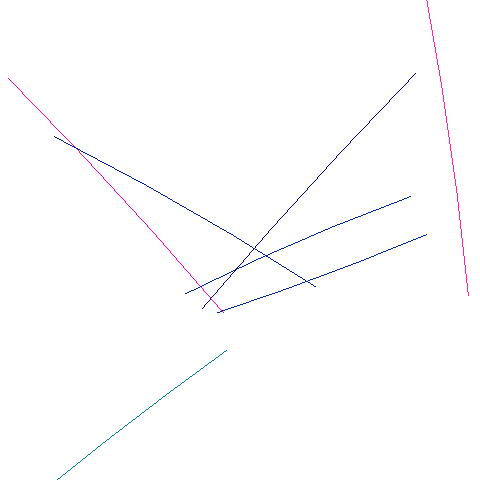
\includegraphics[width=\textwidth]{withAliasing.png}
 		\captionsetup{font={up, footnotesize}}
    	\caption{Widoczny aliasing.}
 		\label{rys25}
	\end{subfigure}
	\hfill
	\begin{subfigure}{0.5\textwidth}
		\centering
		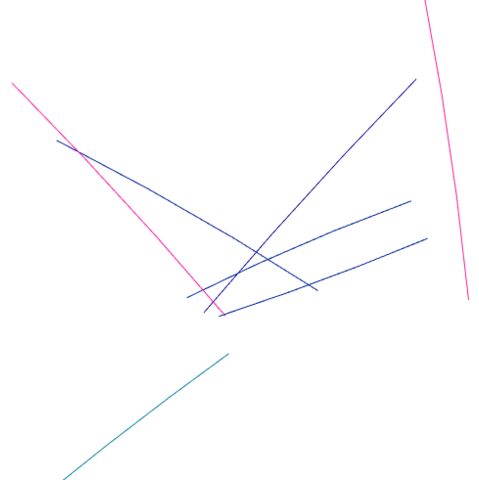
\includegraphics[width=\textwidth]{Antialiasing.png}
		\captionsetup{font={up, footnotesize}}
    	\caption{Po zastosowaniu GLFW\_SAMPLES = 8.}
		\label{rys12}
	\end{subfigure}
	\captionsetup{justification=raggedleft, font={it, footnotesize}}
    \captionsetup{justification=justified, font={up, footnotesize}}
    \caption{Przykład zmniejszenia efektu aliasingu na wyrenderowanych krzywych.}
\vskip\baselineskip
	\begin{subfigure}{0.5\textwidth}
		\centering
 		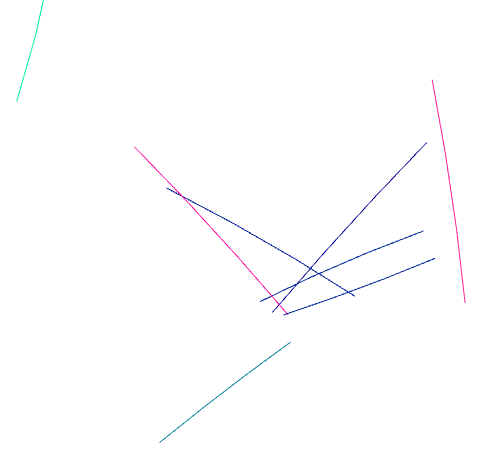
\includegraphics[width=\textwidth]{Wart3.png}
 		\captionsetup{font={up, footnotesize}}
    	\caption{Po zastosowaniu GLFW\_SAMPLES = 3.}
 		\label{rys15}
	\end{subfigure}
	\hfill
	\begin{subfigure}{0.5\textwidth}
		\centering
		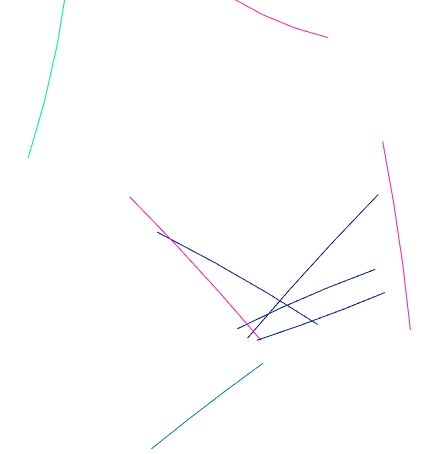
\includegraphics[width=\textwidth]{Wart20.png}
		\captionsetup{font={up, footnotesize}}
    	\caption{Po zastosowaniu GLFW\_SAMPLES = 20.}
		\label{rys16}
	\end{subfigure}
	\captionsetup{justification=raggedleft, font={it, footnotesize}}
    \captionsetup{justification=justified, font={up, footnotesize}}
    \caption{Przykład zmniejszenia efektu aliasingu dla różnych wartości dla GLFW\_SAMPLES.}
    \label{rys17}
\end{figure}

\subsubsection{Rozwiązania alternatywne}

Pierwszym pomysłem na rozwiązanie problemu rysowania wielu cząstek było stworzenie tablicy dwuwymiarowej dla przechowywania informacji o ścieżkach. Określone w ten sposób dane miały spływać do tablic buforów VAO i VBO. W ten sposób tworzyłoby się osobny bufor dla każdego toru. To rozwiązanie jest bardzo naiwne i, mimo że da się dzięki niemu osiągnąć cel --- zwizualizować tory cząstek, nie zostało one użyte.

Głównym zadaniem tych buforów jest przesyłanie paczek danych o wierzchołkach do karty graficznej, żeby nie powtarzać tej samej czynności dla każdego punktu zdefiniowanego w scenie. Pogrupowanie wierzchołków do osobnych buforów dla każdej ścieżki, owszem, zwiększyłoby wydajność w stosunku do przykładu bez buforów, lecz wciąż byłoby zbyt kosztowne.

\subsection{Rysowanie detektora}
\subsubsection{Wczytanie danych z pliku COLLADA}
Do wczytania modelu z dostarczonego pliku w formacie COLLADA użyto biblioteki Assimp. Odbywa się to poprzez ładowanie wszystkich informacji o modelu do uogólnionych struktur danych zdefiniowanych w bibliotece. Po załadowaniu modelu, wszystkie niezbędne do renderowania dane mogą być pobrane ze struktur danych Assimp. Podczas opracowywania programu korzystano z materiałów opublikowanych na stronie internetowej \cite{learnopengl}. 

Pobierany z pliku model jest ładowany do obiektu sceny, przechowującego wszystkie informacje o modelu i jego otoczeniu. Na rysunku \ref{rys14} jest pokazany diagram klas Assimp, definiujący sposób, w jaki odczytanane dane są dzielone i ładowane do pamięci.

Klasa aiScene zawiera wskaźnik do aiNode (węzła głównego sceny), który z kolei utrzymuje wskaźniki do węzłów potomnych. Wskaźnik do aiNode rekursywnie definiuje strukturę sceny. AiScene służy również jako centralne miejsce przechowywania wszystkich siatek, materiałów lub źródeł światła. Natomiast instancje aiNode po prostu indeksują te tablice, które znajdują się w scenie.

Obiekt mMesh przechowuje wszystkie istotne dane wymagane do renderowania: położenia wierzchołków, wektory normalnych, współrzędne tekstur i kształt powierzchni obiektu. Informacje o użytych materiałach można znaleźć w obiekcie klasy aiMaterial. Obiekt klasy aiLight gromadzi informacje o wszystkich źródłach światła w scenie, a w szczególności o ich położeniu, kierunku i kolorach. 

\begin{figure}[H]
		\centering
 		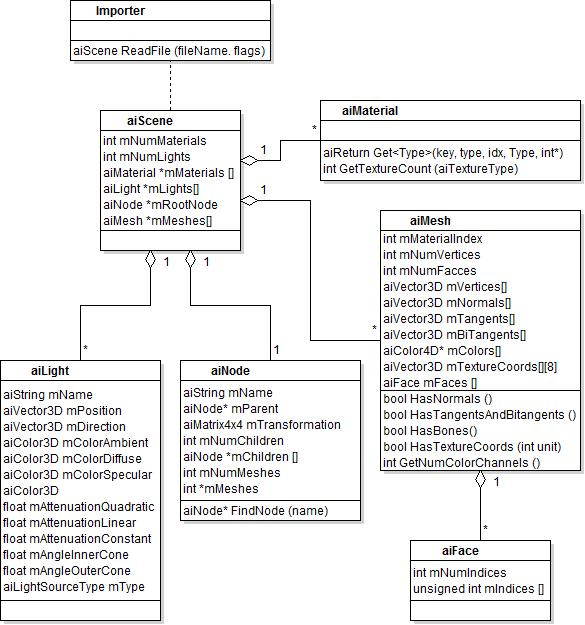
\includegraphics[width=13.0cm]{assimpClasses.png}
 		\captionsetup{font={up, footnotesize}}
    	\caption{Diagram klas sceny wczytanej za pomocą biblioteki Assimp \cite{assimpImport}.}
 		\label{rys14}
\end{figure}

\subsubsection{Określenie siatki detektora}
Użycie biblioteki Assimp daje możliwość załadowania wielu różnych modelów do jednej aplikacji. Jak było wcześniej wspomniane, po wczytaniu wszystkie dane są przechowywane w strukturach Assimp. Dla skorzystania z funkcji renderowania obiektów konieczne jest przekształcenie struktur danych Assimp na struktury w OpenGL.

W rozpatrywanym przypadku pojedyncza encja do narysowania jest reprezentowana przez siatkę (ang. mesh), dlatego rozbudowanie programu zaczęto od zdefiniowania własnej klasy siatki. Składa się ona z zestawu wierzchołków, gdzie każdy wierzchołek zawiera wektory położenia, normalnych.

Klasa Mesh nie jest zbyt skomplikowana (rysunek \ref{rys24}). Założono dość prostą funkcję konstruktora obiektu Mesh, która publiczne zmienne klasy ustawia z odpowiednimi zmiennymi argumentów konstruktora. W argumentach konstruktora są podawane tylko dane podstawowe --- wierzchołki i ich indeksy. Na końcu tej funkcji jest wywoływana metoda setupMesh, która to uzupełnia bufory VAO i VBO w dane. Natomiast bezpośrednie rysowanie siatki odbywa się za pomocą funkcji Draw.

W przypadku rysowania modelu detektora podobnie jak przy tworzeniu obrazu torów cząstek, użyto dodatkowego bufora --- EBO, bufora elementów obiektu (widać to w tabeli \ref{tab12}). Powodem do tego służy fakt, że w modelach przybliżanych siatką trójkątów duża część wierzchołków może się pokrywać. Lepszym rozwiązaniem jest przechowywanie nie wszystkich wierzchołków, a tylko unikatowych, wraz z określaniem kolejności, w której zostaną one wyświetlone \cite{learnopengl}. Również w tym przypadku z pomocą przychodzi bufor elementów obiektu. EBO przechowuje indeksy używane przez OpenGL do podjęcia decyzji, które wierzchołki muszą być wyświetlone i w jakiej kolejności.

\begin{table}[H]
\caption{Kod źródłowy programu. Funkcja definiująca bufory.}
\label{tab12}
\begin{lstlisting}[frame=single]  % Start your code-block

void setupMesh() {
 glGenVertexArrays(1, &VAO);
 glGenBuffers(1, &VBO);
 glGenBuffers(1, &EBO);
 glBindVertexArray(VAO);
 glBindBuffer(GL_ARRAY_BUFFER, VBO);
 glBufferData(GL_ARRAY_BUFFER, vertices.size() * sizeof(Vertex), 
 	&vertices[0], GL_STATIC_DRAW);
 glBindBuffer(GL_ELEMENT_ARRAY_BUFFER, EBO);
 glBufferData(GL_ELEMENT_ARRAY_BUFFER, 
 	indices.size() * sizeof(unsigned int),&indices[0], 
 	GL_STATIC_DRAW);
 glEnableVertexAttribArray(0);
 glVertexAttribPointer(0, 3, GL_FLOAT, GL_FALSE, sizeof(Vertex), 
 	(void*)0);
 glEnableVertexAttribArray(1);
 glVertexAttribPointer(1, 3, GL_FLOAT, GL_FALSE, sizeof(Vertex),
 	(void*)offsetof(Vertex, Normal));
 glBindVertexArray(0);}
\end{lstlisting}
\end{table}

\subsubsection{Wyświetlanie modelu}
Scena może zawierać wiele różnych siatek, dlatego utworzono klasę, która by je łączyła i reprezentowała model w całości (rysunek \ref{rys24}). Z tego powodu w klasie Model został zdefiniowany wektor obiektów typu Mesh --- wektor składający się z różnych siatek odczytanych z pliku. Ładowanie danych z pliku odbywa się za pomocą funkcji loadModel, kod źródłowy tej funkcji jest przedstawiony w tabeli \ref{tab13}.

Początkowo jest tworzony obiekt klasy Importer dedykowany do wczytywania modeli do struktur danych Assimp. Na tym obiekcie wywołano funkcję ReadFile, gdzie jako pierwszy argument jest przyjmowana ścieżka do pliku Collada. Jako drugi argument poprzez funkcję ReadFile są przyjmowane różne opcje używane w trakcie przetwarzania końcowego. Opcje te inicjują dodatkowe obliczenia na odczytanych danych. Ze wszystkimi możliwymi opcjami oraz ich opisami można zapoznać się na stronie z oficjalną dokumentacją biblioteki \cite{assimpDocumentation}.

\begin{table}[H]
\caption{Kod źródłowy programu. Funkcja pobierająca model z pliku.}
\label{tab13}
\begin{lstlisting}[frame=single]  % Start your code-block

void loadModel(string const &path) {
 Assimp::Importer importer;
 const aiScene* scene = importer.ReadFile(path, aiProcess_Triangulate);
 if(!scene || scene->mFlags || !scene->mRootNode) {
  cout << "ERROR::ASSIMP::" << importer.GetErrorString() << endl;
  return; }
  processNode(scene->mRootNode, scene); }
\end{lstlisting}
\end{table}

Jak było pokazane na diagramie klas (rysunek \ref{rys14}) scena w Assimp ma strukturę drzewiastą. Po wczytaniu sceny przetwarzane są wszystkie jej węzły, służy do tego rekursywna funkcja processNode, która zatrzymuje swoje działanie dopiero w chwili, gdy wszystkie węzły sceny zostały już przetworzone (tabela \ref{tab18}). Na tym etapie zostaje uzupełniony w dane wektor siatek.

\begin{table}[H]
\caption{Kod źródłowy programu. Funkcja przetwarzająca węzły sceny.}
\label{tab18}
\begin{lstlisting}[frame=single]  % Start your code-block

void processNode(aiNode *node, const aiScene *scene){
 for(unsigned int i = 0; i < node->mNumMeshes; i++){
  aiMesh* mesh = scene->mMeshes[node->mMeshes[i]];
  meshes.push_back(processMesh(mesh, scene));}
 for(unsigned int i = 0; i < node->mNumChildren; i++){
   processNode(node->mChildren[i], scene);}}
\end{lstlisting}
\end{table}

Samo przetwarzanie siatki sprowadza się do 2 czynności: do pobierania wszystkich informacji o wierzchołkach oraz do pobierania indeksów siatki. Na koniec wywoływany jest konstruktor obiektu Mesh. W tabeli \ref{tab14} z kodem źródłowym pokazana jest funkcja przetwarzająca siatki w modelu.

Pobieranie informacji o wierzchołkach zostało zrealizowane poprzez zdefiniowanie struktury wierzchołków, która po każdej iteracji jest dodawana do ogólnej tablicy wierzchołków. Do załadowania danych o indeksach siatki skorzystano z interfejsu udostępnionego przez bibliotekę Assimp --- aiFace. Face, w kontekście opracowywanego programu, jest najmniejszym zdefiniowanym prymitywem i ma on kształt trójkąta. Ten właśnie prymityw przechowuje indeksy definiujące kolejność wyświetlania wierzchołków siatki.

Na podstawie uzyskanych danych z Assimp --- listy wierzchołków i indeksów --- uruchomiono pętlę rysującą siatkę. Do rysowania użyto funkcji glDrawElements, tak samo, jak w przypadku torów cząstek.

\begin{table}[H]
\caption{Kod źródłowy programu. Funkcja przetwarzania siatek w modelu.}
\label{tab14}
\begin{lstlisting}[frame=single]  % Start your code-block

Mesh processMesh(aiMesh *mesh, const aiScene *scene) {
 vector<Vertex> vertices;
 vector<unsigned int> indices;
 for(unsigned int i = 0; i < mesh->mNumVertices; i++) {
  Vertex vertex;
  glm::vec3 vector;
  vector.x = mesh->mVertices[i].x;
  vector.y = mesh->mVertices[i].y;
  vector.z = mesh->mVertices[i].z;
  vertex.Position = vector;
  vector.x = mesh->mNormals[i].x;
  vector.y = mesh->mNormals[i].y;
  vector.z = mesh->mNormals[i].z;
  vertex.Normal = vector;
  vertices.push_back(vertex);}
 for(unsigned int i = 0; i < mesh->mNumFaces; i++) {
  aiFace face = mesh->mFaces[i];
  for(unsigned int j = 0; j < face.mNumIndices; j++)
   indices.push_back(face.mIndices[j]); }
 return Mesh(vertices, indices);}
\end{lstlisting}
\end{table}

\subsubsection{Napotkane problemy}
Przed rozpoczęciem prac nad programem wizualizacji detektora zakładano, że geometria modelu zostanie bezpośrednio pobrana z repozytorium w CERN. Okazało się jednak, że nie są to szeroko dostępne dane oraz że są one przechowywane w strukturach danych biblioteki ROOT.

ROOT również posiada własną platformę graficzną (ROOT 3D Graphics: TGeoManager \cite{root3dGraphics}) umożliwiającą tworzenie obrazów na podstawie przeanalizowanych danych. W tej oto platformie początkowo stworzono model detektora ALICE. Bezpośrednie pobranie danych o modelu wiązałoby się z dużym nakładem prac w kierunku przestudiowania struktur danych ROOT 3D Graphics i stworzenia odpowiedniego programu do przekształcenia danych na konkretny format pliku 3D (na przykład .obj czy .dae).

Potrzebne rozwiązanie już zostało opracowane w CERN, ale nie zostało jeszcze upublicznione, dlatego na potrzeby niniejszej pracy inżynierskiej otrzymano gotowy plik COLLADA z geometrią detektora ALICE. Ze względu na to, że niezbędne oprogramowanie jest w trakcie tworzenia, otrzymany plik zawierał błędy w strukturze formatu. Ujawniało się to między innymi podczas ładowania modelu z pliku do obiektu aiScene.

Przy uruchomieniu programu pojawiał się komunikat o błędzie: \textquotedblleft ERROR::ASSIMP:: Collada: aliceGeom.dae - Expected end of <accessor> element \textquotedblright . Ta wiadomość jest generowana przez funkcję readAccessor w pliku ColladaParser.kt (biblioteka Assimp) i świadczy o błędzie składni podczas użycia funkcji COLLADA <accessor>/<param> \cite{collada}.

Rozwiązano ten problem za pomocą narzędzia Blender, do którego najpierw wczytano nie do końca poprawny plik z modelem detektora, a później wyeksportowano ten sam model do innego pliku, również z rozszerzeniem .dae. Po wykonaniu tych prostych czynności udało się wyświetlić geometrię detektora ALICE.

Jednak niepoprawna struktura pliku COLLADA przełożyła się również na współrzędne użytych materiałów. Tych danych już niestety nie udało się naprawić w dostępnych programach graficznych. Dlatego wczytaną siatkę modelu pokolorowano w jeden podstawowy kolor (niebieski). Na rysunku \ref{rys28} widać kształt detektora, lecz z braku możliwości wglądu w warstwy wewnętrzne i braku poprawnych materiałów, obraz ten wygląda prymitywnie.

\begin{figure}[H]
		\centering
 		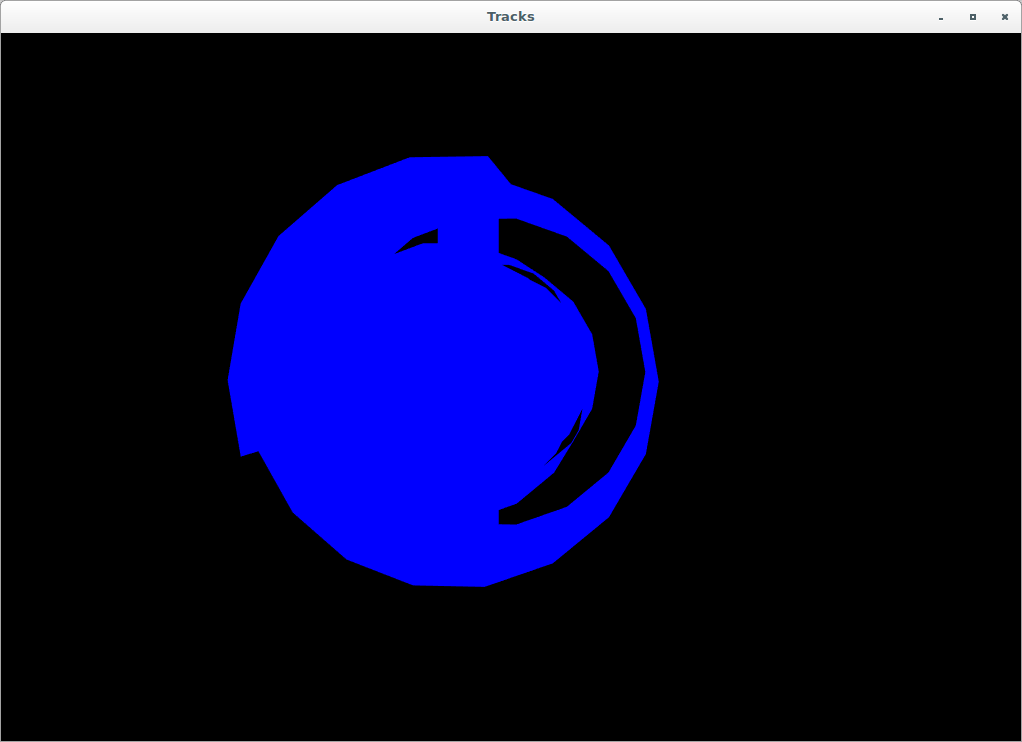
\includegraphics[width=12.0cm]{myGeom.png}
 		\captionsetup{font={up, footnotesize}}
    	\caption{Obraz detektora}
 		\label{rys28}
\end{figure}

\subsection{Tworzenie obrazu stereoskopowego w technice pasywnej}
Pasywne wizualizacje stereoskopowe wymagają przygotowanych wcześniej dwóch obrazów z różniącą się perspektywą i umieszczenia tych obrazów obok siebie. Dla stworzenia różniących się perspektyw w OpenGL muszą być dopasowane regulacja asymetryczna wraz z widokiem renderowanego obszaru. Obszar widoku jest równoległym rzutem asymetrycznym w kształcie ściętego stożka lub równoważnym przesunięciem obiektywu w fotografii.

Opisywana technika nie wprowadza pionowej paralaksy i jest powszechnie stosowana w renderowaniu stereoskopowym \cite{openglCookbook}. Do zilustrowania koncepcji dla prawego oka (dla lewego oka są wykonywane analogiczne transformacje w lustrzanym odbiciu) wykorzystano rysunek \ref{rys10}. Przesunięcie reprezentuje wielkość odchylenia dla regulacji asymetrycznej ściętego stożka.

\begin{figure}[H]
		\centering
 		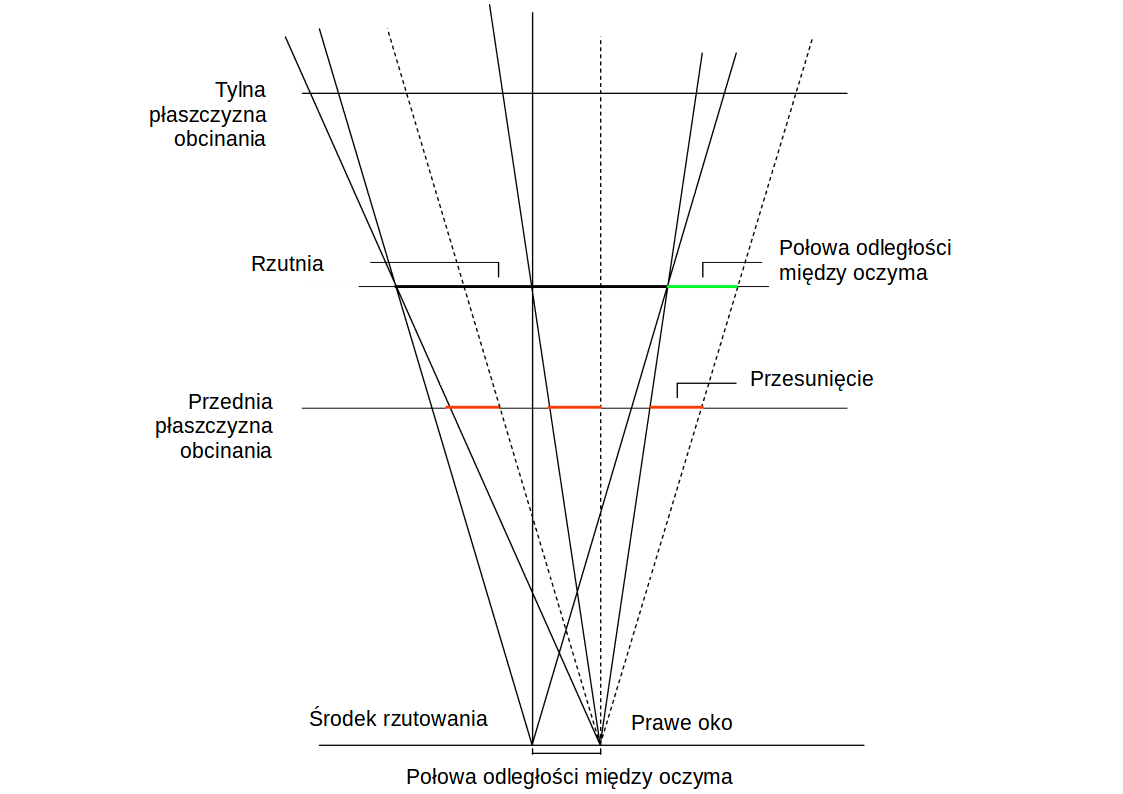
\includegraphics[width=12cm]{stereoscopicGL.png}
 		\captionsetup{font={up, footnotesize}}
    	\caption{Geometria sceny, którą użytkownik widzi z perspektywy prawego oka \cite{openglCookbook}.}
 		\label{rys10}
\end{figure}

Kod źródłowy umieszczony w tabeli \ref{tab5} przedstawia implementację tworzenia rzutowania i wyświetlania macierzy dla wizualizacji stereoskopowej. Kod wykorzystuje odległość między oczyma (zmienna IOD w kodzie), odległość płaszczyzny obrazu (zmienna depthZ) oraz odległość bliskiej płaszczyzny rzutowania (zmienna nearZ). Wymienione zmienne są użyte do określenia wartości przesunięcia (zmienna frustumshift). W przedstawionym kodzie źródłowym są zaimplementowane również obliczenia macierzy projekcji i widoku, skorzystano do tego z funkcji biblioteki GLM, podobnie jak w przypadku ze zwykłą kamerą dla widoku była to funkcja glm::lookAt. Natomiast macierz projekcji obliczano za pomocą funkcji glm::frustum;

W tabeli \ref{tab10} zaprezentowano implementację stworzenia obrazów dla każdego oka, poprzez odpowiednie ustawienia macierzy projekcji i widoku. Dla każdego oka położenie kamery jest przesuwane o połowę odległości między oczyma (jak zostało pokazane na rys. \ref{rys10}).

Kod źródłowy w tabelach \ref{tab5} i \ref{tab10} był stworzony na podstawie \cite{openglCookbook}. Ostateczny wynik renderowania składa się z dwóch oddzielnych obrazów po obu stronach ekranu.

\newpage
\begin{table}[H]
\caption{Kod źródłowy programu. Implementacja przekształceń macierzy stereoskopowych.}
\label{tab5}
\begin{lstlisting}[frame=single]  % Start your code-block

void computeStereoView(float aspect_ratio, float IOD, float depthZ, 
  bool left_eye, glm::vec3 up = glm::vec3(0.0f, 100.0f, 0.0f), 
  glm::vec3 direction_z = glm::vec3(0, 0, 1) ) {
  float left_right_direction = -1.0f;
  if (left_eye)
     left_right_direction = 1.0f;
  double frustumshift = (IOD / 2) * nearZ / depthZ;
  float top = tan(g_initial_fov / 2.0f) * nearZ;
  float right = aspect_ratio * top + frustumshift * left_right_direction;
  float left = -aspect_ratio * top + frustumshift * left_right_direction;
  float bottom = -top;
  g_projection_matrix = glm::frustum(left,right,bottom,top,nearZ,farZ);
  g_view_matrix = glm::lookAt( g_position - direction_z + 
  	glm::vec3(left_right_direction * IOD / 2, 0, 0),
    g_position + glm::vec3(left_right_direction * IOD / 2, 0, 0), up); }
\end{lstlisting}
\end{table}
\begin{table}[H]
\caption{Kod źródłowy programu. Implementacja ustawień macierzy projekcji i widoku.}
\label{tab10}
\begin{lstlisting}[frame=single]  % Start your code-block

void drawStereo (glm::mat4 transform, Shader shader, int trackSize,
 Track track ) {
 glm::mat4 projection = glm::perspective(glm::radians(camera.Zoom),
     (float)SCR_WIDTH / (float)SCR_HEIGHT, 0.1f, 100.0f);
 shader.setMat4("projection", projection);
 glm::mat4 view = camera.GetViewMatrix();
 shader.setMat4("view", view);
 glm::mat4 model = glm::mat4(1.0);
 transform = glm::scale(transform, glm::vec3(0.01, 0.01, 0.01));
 transform = glm::translate(model, glm::vec3(0.0f, 0.0f, -depthZ));
 transform = glm::rotate(model, glm::pi<float>() * rotateY, 
     glm::vec3(0.0f, 1.0f, 0.0f));
 transform = glm::rotate(model, glm::pi<float>() * rotateX, 
     glm::vec3(1.0f, 0.0f, 0.0f));
 GLint transformLoc = glGetUniformLocation(shader.ID, "transform");
 glUniformMatrix4fv(transformLoc, 1, GL_FALSE, glm::value_ptr(transform));
track.draw(); }
\end{lstlisting}
\end{table}


\subsection{Tworzenie aktywnego obrazu stereoskopowego} 
W trakcie opracowania oprogramowania wizualizacji stereoskopowych został zaprojektowany algorytm dla aktywnej techniki stereoskopowej. Algorytm ten składa się z 8 kroków, które należy zapętlić:

\begin{itemize}
\itemi Ustawienie widoku dla lewego oka.
\itemi Załadowanie widoku dla lewego oka do bufora.
\itemi Wyświetlenie widoku dla lewego oka.
\itemi Czyszczenie Z-bufora (jeśli używany jest ten sam dla lewego i prawego obrazu).
\itemi Ustawienie widoku dla prawego oka.
\itemi Załadowanie widoku dla prawego oka do bufora.
\itemi Wyświetlenie widoku dla prawego oka.
\itemi Wymiana buforów.
\end{itemize}

Wszystkie działania algorytmu należałoby wykonywać z bardzo dużą częstotliwością, co najmniej 120 razy na sekundę.

Użycie takiego algorytmu jest dobre tylko w teorii, gdyż w rzeczywistości powstaje problem synchronizacji wyświetlacza i okularów 3D. W zestawie Nvidia 3D Vision ten problem jest rozwiązany na poziomie sprzętowym, użyto do tego nadajnika podczerwieni oraz specjalnych okularów.

Niestety, w roku 2008 firma Nvidia usunęła stereoskopową obsługę OpenGL dla kart graficznych GeForce i AMD. Jednak była kontynuowana obsługa wyświetlania obrazów stereoskopowych z OpenGL w najdroższych, profesjonalnych rozwiązaniach Quadro + 3D Vision. Ten niefortunny stan rzeczy zmienił się w lutym 2013 roku, przy realizacji kolejnego sterownika Nvidia GeForce 314.07. Biblioteka OpenGL zaczęła działać dla pełnoekranowych programów stereoskopowych dla pojedynczych konfiguracji komputerowych (na przykład Windows 8 64-bit, GeForce GTX 680M). Wszystkie informacje o konfiguracjach można znaleźć na oficjalnym formum użytkowników GeForce \cite{GeForceForum}.

Zmiana, która zaszła, nie była zapowiedziana oficjalnie i mogła ona być niezamierzonym efektem wprowadzonych do sterownika modyfikacji, a powodzenie przy uruchomieniu OpenGL na wybranych konfiguracjach komputerów i zastawów 3D Vision można uważać za wyjątek. Z informacji umieszczonych na oficjalnej stronie internetowej \cite{NvidiaInfo} wynika, że ta technologia wciąż nie wspiera biblioteki OpenGL. Stąd, osiągnięcie celu: wykonanie obrazów w technologii stereoskopii aktywnej, nie jest możliwe.

Gry komputerowe, które można wyświetlać za pomocą zestawu do stereoskopii aktywnej, są tworzone przy użyciu silnika gragicznego Unity w wersjach 4 Pro lub 5. Dla połącznia Unity z 3D Vision została opracowana specjalna wtyczka, którą można kupić na stronie \cite{Unity}.

W ramach opracowania uruchomiono zestaw Nvidia 3D Vision z programami dostarczonymi w pakiecie. Podczas uruchomienia należy krok po kroku spełniać wszystkie wymagania spisane na stronie \cite{NvidiaInfo}, w przeciwnym przypadku grozi to niepowodzeniem w próbach skonfigurowania sprzętu z oprogramowaniem.

\newpage
\subsection{Weryfikacja poprawności i jakości programu}
Weryfikacja poprawności i jakości programu może mieć różny charakter i odnosić się do różnych etapów procesu wytwórczego. W działaniach weryfikacyjnych w niniejszej pracy dyplomowej posługiwano się wskazówkami z książki \cite{specyfikacja}.

Po zakończeniu procesu wytwórczego oceniono końcowy produkt --- program wraz z jakością stworzonych obrazów. Zwrócono uwagę również na stopień spełnienia przez oprogramowanie wymagań funkcjonalnych i niefunkcjonalnych.

\begin{table}[H]
\caption{Stopień spełnienia wymagań funkcjonalnych.}
\centering
\footnotesize
\label{tab15}
\begin{tabular}{!{\color{sapphire}\vrule width 1pt}m{0.05\textwidth}!{\color{black}\vrule width 1pt}m{0.26\textwidth}!{\color{black}\vrule width 1pt}m{0.57\textwidth}!{\color{sapphire}\vrule width 1pt}}
	\arrayrulecolor{sapphire}\hline
	\Centering\bfseries Nr &
	\Centering\bfseries Nazwa &
	\Centering\bfseries W jakim stopniu jest spełnione \\
	\hline
	\arrayrulecolor{black}
	1 & Renderowanie torów cząstek & Spełnione w 100\%, obrazy umieszczono w Dodatku \ref{Tory}.\\ 
	\hline
	2 & Renderowanie detektora & Spełnione w 100\%.\\ 
	\hline
	3 & Stworzenie efektu widzenia stereoskopowego & Spełnione w 100\%. Przetestowano w laboratorium graficznym z użyciem zestawu 3D.\\ 
	\hline
	4 & Stworzenie efektu aktywnego widzenia stereoskopowego &  Nie spełniono, ze względu na ograniczenia sprzętowe.\\ 
	\hline
	5 & Możliwość interakcji z użytkownikiem & Spełnione w 100\%, instrukcję użytkownika umieszczono w folderze z kodem źródłowym. \\ 
	\arrayrulecolor{sapphire}\hline
\end{tabular}
\end{table}

\begin{table}[H]
\caption{Stopień spełnienia wymagań niefukcjonalnych.}
\centering
\footnotesize
\label{tab19}
\begin{tabular}{!{\color{sapphire}\vrule width 1pt}m{0.05\textwidth}!{\color{black}\vrule width 1pt}m{0.26\textwidth}!{\color{black}\vrule width 1pt}m{0.57\textwidth}!{\color{sapphire}\vrule width 1pt}}
	\arrayrulecolor{sapphire}\hline
	\Centering\bfseries Nr &
	\Centering\bfseries Nazwa &
	\Centering\bfseries W jakim stopniu jest spełnione \\
	\hline
	\arrayrulecolor{black}
	1 & Przenośność & Spełnione w 100\%. Program bezproblemowo uruchamiano na różnych systemach operacyjnych.\\ 
	\hline
	2 & Zrozumiałość & Spełnione w 100\%, instrukcję użytkownika umieszczono w folderze z kodem źródłowym.. \\ 
	\hline
	3 & Czytelność kodu źródłowego & Spełnione w 70\%, niektóre rozwiązania niezgodne z zasadami czystego kodu zastosowano ze względu na specyfikacje bibliotek zewnętrznych. \\ 
	\hline
	4 & Tolerowanie defektów & Spełnione w 100\%, błędne dane mogą być wprowadzone tylko poprzez pliki zewnętrzne. O problemach z plikiem użytkownik zostanie poinformawany za pomocą komunikatów błędu, odpowiednich dla analizatorów składni wybranego formatu. \\
	\hline
	5 & Przyjazność programu dla użytkownika & Spełnione w 100\%, instrukcję użytkownika umieszczono w folderze z kodem źródłowym.\\  
	\arrayrulecolor{sapphire}\hline
\end{tabular}
\end{table}


\subsection{Porównanie technologii stereoskopowych}
Po przetestowaniu oprogramowania na dwóch zestawach dla widzenia stereoskopowego można wyciągnąć pewne wnioski, a przede wszystkim mieć podstawy i kryteria do porównania technologii widzenia w trzech wymiarach.

Pierwsza rzecz, na którą zwraca się uwagę podczas pierwszego korzystania z zestawów, to znacząca różnica w rozdzielczości. Stereoskopia aktywna jest bezwarunkowo w tym lepsza od technologii pasywnej.

Kolejna ważna rzecz to jasność obrazu. Po założeniu okularów zauważalny jest spadek jasności niemal o połowę. W przypadku obu metod, zarówno aktywnej, jak i pasywnej, tylko połowa światła dociera do oka. W technologii aktywnej jest to spowodowane przyciemnianiem soczewek na zmianę, w przypadku pasywnego 3D co druga wyświetlana przez ekran linia jest czarna. Aby zrekompensować tę stratę, większość wyświetlaczy po prostu zwiększa jasność w trybie stereoskopowym.

Obie wyżej wymienione własności mają wpływ na jakość obrazu i na komfort oglądania. Biorąc pod uwagę to kryterium, warto odznaczyć, że każda technologia ma wady, których nie da się wyeliminować, gdyż leżą one u podstaw działania technik. W przypadku stereoskopii pasywnej wadą jest dobranie odpowiedniej pozycji, żeby móc obejrzeć obraz stereoskopowy. Wiąże się to, z dopasowaniem polaryzacji ekranu i okularów, ponieważ każde odchylenie zaburza cały obraz. W przypadku stereoskopii aktywnej komfort oglądania zaburzają migotanie obrazu. Migotanie jest spowodowane szybką zmianą obrazów i przyciemnianiem odpowiednich soczewek. Po dłuższym oglądaniu wada ta może doprowadzić do bólu głowy, a w przypadkach skrajnych nawet do ataku epileptycznego. Dlatego przed użyciem Nvidia 3D Vision należy wykonać test zdrowotny, udostępniony w oprogramowaniu zestawu, który sprawdza podatność organizmu na efekty uboczne.

Jak technika stereoskopowego widzenia pasywnego, tak i aktywnego wymagają użycia okularów. Wadą okularów aktywnych jest po pierwsze koszt, a po drugie bateria, która musi być naładowana, żeby oglądanie obrazów trójwymiarowych się powiodło. Warto zaznaczyć, że urządzenia umożliwiające widzenie stereoskopowe stają się coraz bardziej popularne, lecz nie są jeszcze powszechnie dostępne w sklepach.

Tabela \ref{tab19} strukturyzuje opisane wcześniej informacje.

\begin{table}[H]
\caption{Porównanie technologii stereoskopowych.}
\centering
\footnotesize
\label{tab19}
\begin{tabular}{!{\color{sapphire}\vrule width 1pt}m{0.29\textwidth}!{\color{black}\vrule width 1pt}m{0.29\textwidth}!{\color{black}\vrule width 1pt}m{0.29\textwidth}!{\color{sapphire}\vrule width 1pt}}
	\arrayrulecolor{sapphire}\hline
	\Centering\bfseries Kryterium &
	\Centering\bfseries Stereoskopia pasywna &
	\Centering\bfseries Stereoskopia aktywna \\
	\hline
	\arrayrulecolor{black}
	Rozdzielczość & Średnia: 1920x540 & Bardzo wysoka: 1920x1080. \\ 
	\hline
	Jasność & Słaba & Słaba \\ 
	\hline
	Komfort oglądania & Trzeba utrzymywać stałe położenie przy ekranie. & Migotanie może powodować ból głowy. \\
	\hline
	Dostępność na rynku & Średnia & Średnia \\
	\hline
	Okulary & Niedrogie, nie wymagają baterii. & Drogie, wymagają posiadanie naładowanej baterii.  \\  
	\arrayrulecolor{sapphire}\hline
\end{tabular}
\end{table}

Pomimo wielu zalet stereoskopii pasywnej, finalnie oddano przewagę technologii aktywnej ze względu na rozdzielczość obrazu i na komfort użycia. Przy oglądaniu do 30 minut nie było objaw żadnego efektu ubocznego i też nie było problemów z wybraniem położenia przy ekranie.

\newpage
\section{Podsumowanie}
Opracowanie wizualizacji stereoskopowych detektora ALICE wymagało podzielenia całości prac na kilka dużych etapów.

Określenie celów całego przedsięwzięcia na samym początku wyznaczyło kierunek rozwoju opracowania, wyeliminowało ścieżki alternatywne, narzucając z góry OpenGL jako podstawową bibliotekę graficzną. Etap pozwolił naszkicować ogólny plan postępowania w dążeniu za wizją niniejszej pracy dyplomowej --- zwiększeniu atrakcyjności fizyki dużych energii poprzez obrazy stereoskopowe.

Znaczącą częścią tego opracowania jest etap analizy, zaczynając od przestudiowania dostępnych technik stereoskopowych aż po poznanie eksperymentów z cząstkami w międzynarodowym laboratorium fizyki cząstek CERN. Już na tym etapie powstał pewien problem nie do ominięcia. Jak to było opisywane wcześniej, pobranie danych z repozytoriów w laboratorium ALICE sprowadziłoby się do stworzenia skomplikowanego parsera plików w języku ROOT. Dlatego, mimo że nie było to bezpośrednim celem niniejszej pracy, przeanalizowano różne formaty plików 3D oraz biblioteki, które by były w stanie wczytać modele z tych plików do sceny w programie. Dzięki takiej analizie stało się możliwe wykonanie zapytania o model w najbardziej pasującym rozszerzeniu (.DAE). Po części analitycznej zaczęto projektowanie oprogramowania.

Proces projektowania w całości przebiegał zgodnie z zaleceniami z \cite{specyfikacja}. Po ogólnym opisie projektu wyspecyfikowano wymagania funkcjonalne i niefunkcjonalne, określono przypadki użycia.

Lukę między opisem wymagań a implementacją wypełnił projekt oprogramowania, definiujący jego elementy składowe oraz ich zachowanie. Wyznaczony schemat, zgodnie z którym zostały napisane i uruchomione wszystkie metody, zaplanowano i opisano w diagramie klas. Na tym etapie również określono biblioteki do użycia w programie. Opracowany projekt był dużym wsparciem podczas implementacji rozwiązania, gdyż pozwalał kontrolować przebieg prac oraz utrzymywać jakość produktu końcowego na odpowiednim poziomie.

Kolejnym ważnym etapem była implementacja zaprojektowanego programu. W tej części opracowania prowadzono najwięcej eksperymentów z różnymi wartościami mającymi wpływ na jakość tworzonych obrazów. Ponadto dużą składową etapu implementacji było testowanie. Celem testowania było doświadczalne porównanie programu z projektem. Integralną częścią weryfikacji poprawności programu było wyświetlenie obrazów końcowych z użyciem różnego sprzętu komputerowego i stereoskopowego. Testowanie oprogramowania zakończono pomyślnie, oznacza to, że produkt końcowy spełnia wymagania projektowe i dodatkowo jest atrakcyjny pod względem technologii, z których korzysta.

Tak jak przy przygotowaniu przeważnej większości opracowań informatycznych, tak i w niniejszym pojawiały się rozmaite trudności, których nie przewidziano wcześniej. Wbrew tym niedogodnościom zrealizowano większość celów. Reasumując założenia wstępne to:
\begin{itemize}
\itemi analiza dostępnych narzędzi graficznych;
\itemi stworzenie oprogramowania z wykorzystaniem biblioteki OpenGL, które:
\begin{itemize}
\itemii wyświetla detektor ALICE;
\itemii zobrazowuje zderzenia cząstek w eksperymencie ALICE;
\end{itemize}
\itemi osiągnięcie efektu głębi w stworzonych obrazach za pomocą dwóch technologii;
\itemi zapewnienie przenośności oprogramowania (działa zarówno pod systemem operacyjnym Linux, jak i Windows).
\end{itemize}

Nie do końca został zrealizowany cel różnorodności technologii stereoskopowych. Jest to związane z wymaganiami systemowymi obsługi stereoskopii aktywnej. Obecnie liderem na rynku aktywnych obrazów stereoskopowych jest technologia Nvidia 3D Vision, która nie wspiera jeszcze biblioteki OpenGL. Natomiast pozostałe cele zostały w pełni zrealizowane. 

\subsection{Ciąg dalszy prac}
Wizualizacje 3D w nauce są bardzo obiecującym obszarem zastosowania. W kolejnym opracowaniu temat stereoskopii zostałby rozszerzony do wirtualnej rzeczywistości. Wtedy zestaw VR (ang. Virtual Reality, wirtualna rzeczywistość) oferowałby szansę zobaczenia akceleratora LHC, detektorów i centrum danych z bliska.

Obecnie potężne aplikacje do wizualizacji naukowych mogą być rozwijane przy użyciu istniejących technologii dość małym kosztem. Tendencja do projektowania zwykłych komputerów w kierunku szybszej grafiki, większej mocy obliczeniowej, systemów operacyjnych wspierających współbieżność i bardzo dużej pamięci powinna wesprzeć i przyspieszyć rozwój rzeczywistości wirtualnej.

Wykorzystanie najnowszych technologii skróciłoby dystans między złożoną terminologią naukową a szerokim zrozumieniem społecznym. Poprzez zanurzenie publiczności do w pełni interaktywnego środowiska można by wizualizować trudne pojęcia fizyczne. Wypełniłoby to lukę między nauką, interaktywnymi mediami i wizualizacją informacji.

\subsection{Zakończenie}
Wizualizacje trójwymiarowe w celach dydaktycznych czy naukowych stanowią nieoceniony napęd w rozwoju komputerów i nowych technologii.   Tak duży postęp narzędzi multimedialnych w ostatnich czasach sprawia, że coraz częściej wizualizacje trójwymiarowe można powszechnie spotkać na uczelniach lub w centrach rozrywki.

Oczywiście obrazy trójwymiarowe przedstawiane na zwykłym ekranie 2D bez zastosowania sprzętu specjalistycznego (okularów 3D, emitera podczerwieni w przypadku stereoskopii aktywnej) są prymitywną symulacją, przedstawieniem sceny trójwymiarowej na płaszczyźnie o dwóch wymiarach. Jednak poprzez połączenie technologii stereoskopowych z animacją można uzyskać kolosalne narzędzie edukacyjne, które by było potężnym wsparciem dla stosowanych w tej chwili metodyk. 

\begin{appendices}
\section{Wyniki tworzenia obrazów torów cząstek}
\label{Tory}
\begin{figure}[H]
	\begin{subfigure}{0.50\textwidth}
		\centering
 		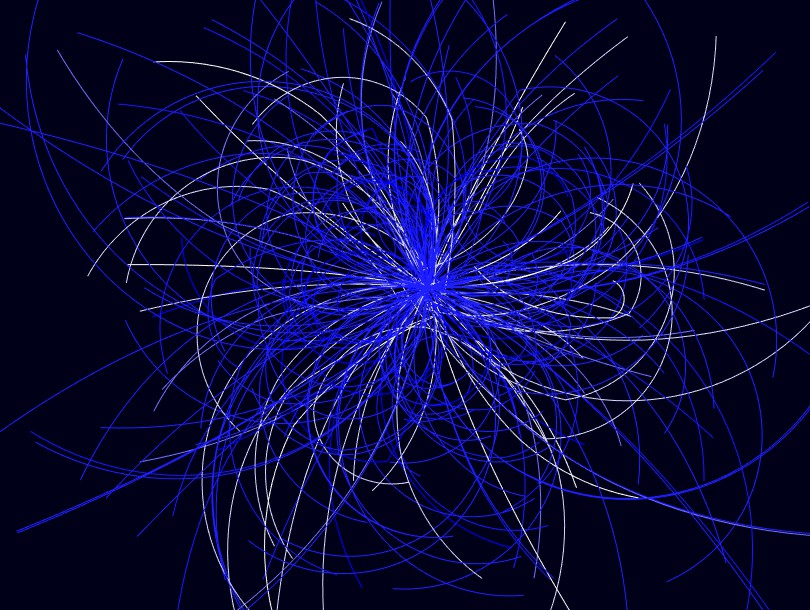
\includegraphics[width=\textwidth]{TrackScreen7.jpg}
 		\captionsetup{font={up, footnotesize}}
    	\caption{Dane z pliku event4047\_run226466.json}
 		\label{rys18}
	\end{subfigure}
	\hfill
	\begin{subfigure}{0.50\textwidth}
		\centering
		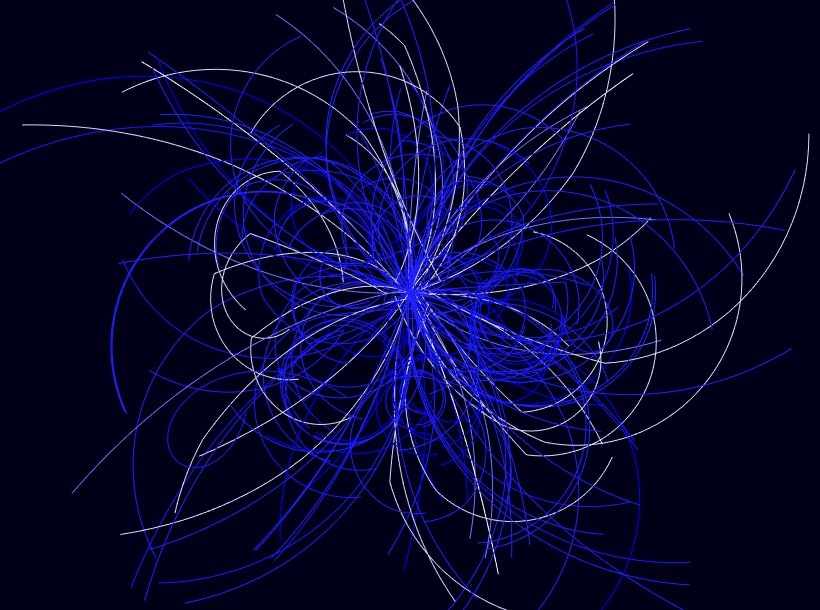
\includegraphics[width=\textwidth]{TrackScreen3.jpg}
		\captionsetup{font={up, footnotesize}}
    	\caption{Dane z pliku event254\_run226466.json}
		\label{rys19}
	\end{subfigure}	
	\vskip\baselineskip
		\begin{subfigure}{0.50\textwidth}
		\centering
 		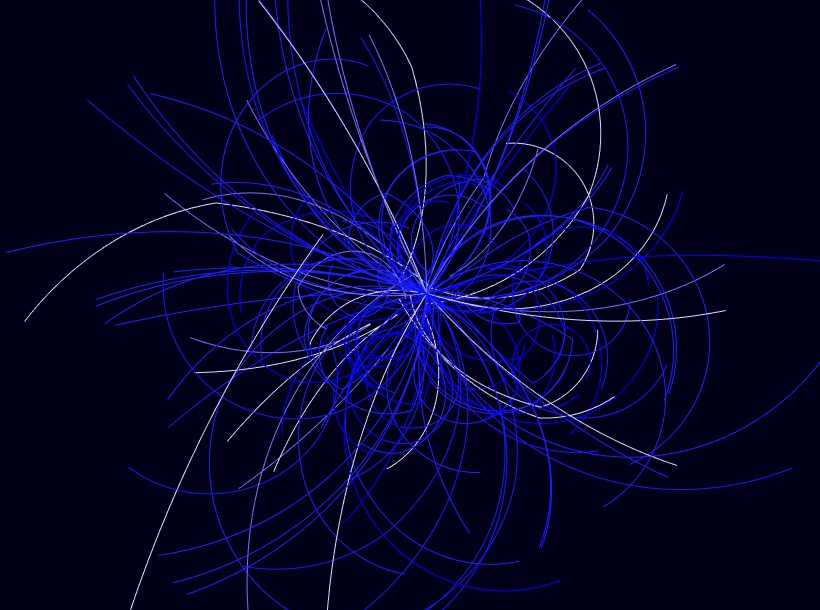
\includegraphics[width=\textwidth]{TrackScreen4.jpg}
 		\captionsetup{font={up, footnotesize}}
    	\caption{Dane z pliku event786\_run122374.json}
 		\label{rys20}
	\end{subfigure}
	\hfill
	\begin{subfigure}{0.50\textwidth}
		\centering
		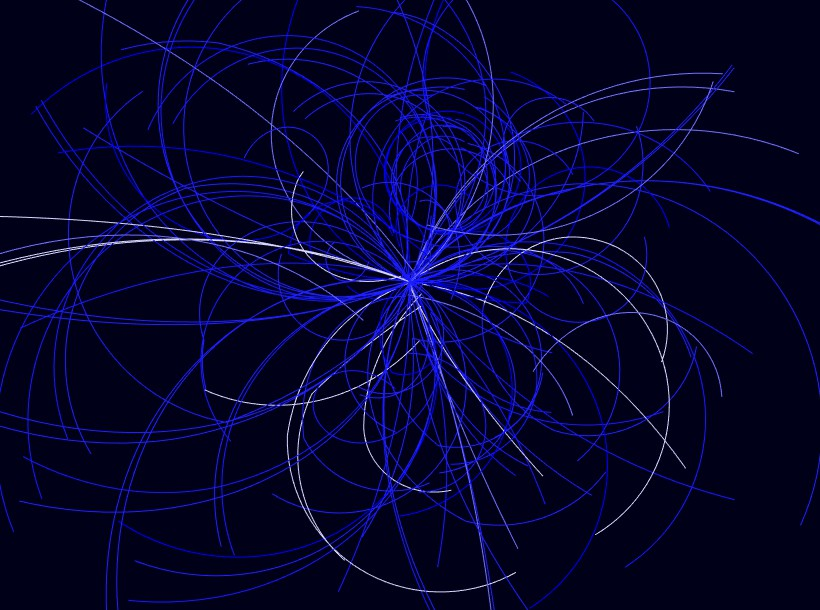
\includegraphics[width=\textwidth]{TrackScreen5.jpg}
		\captionsetup{font={up, footnotesize}}
    	\caption{Dane z pliku event1153\_run122374.json}
		\label{rys21}
	\end{subfigure}
	
	\vskip\baselineskip
		\begin{subfigure}{0.50\textwidth}
		\centering
 		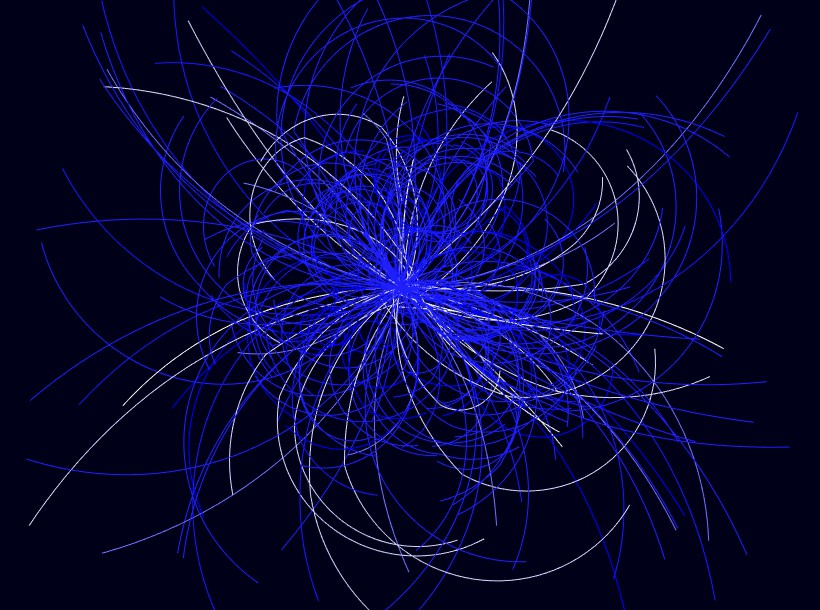
\includegraphics[width=\textwidth]{TrackScreen6.jpg}
 		\captionsetup{font={up, footnotesize}}
    	\caption{Dane z pliku event2162\_run226466.json}
 		\label{rys22}
	\end{subfigure}
	\hfill
	\begin{subfigure}{0.50\textwidth}
		\centering
		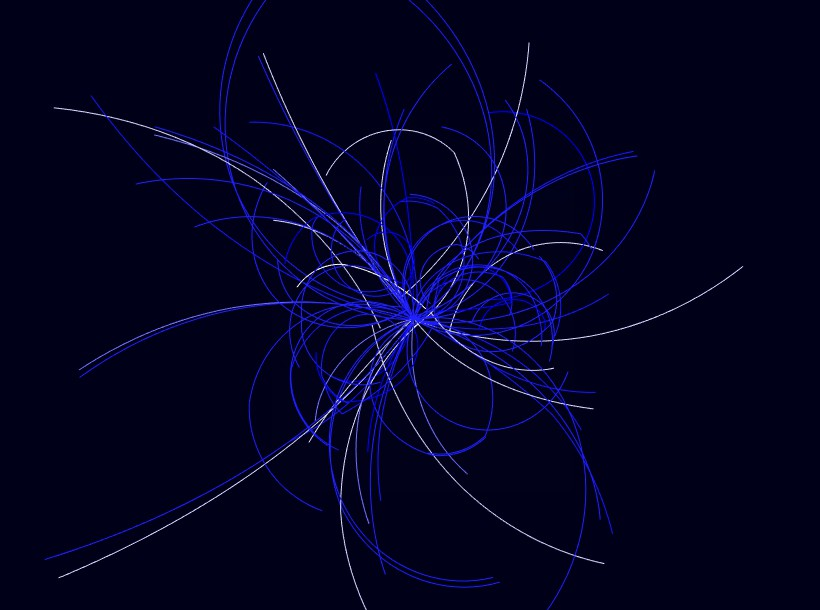
\includegraphics[width=\textwidth]{TrackScreen1.jpg}
		\captionsetup{font={up, footnotesize}}
    	\caption{Dane z pliku event3055\_run226466.json}
		\label{rys23}
	\end{subfigure}
    \label{rys30}
\end{figure}

\newpage
\section{Wyniki tworzenia obrazów dla stereoskopii pasywnej}
\label{sideBside}
\begin{figure}[H]
	\begin{subfigure}{0.90\textwidth}
		\centering
 		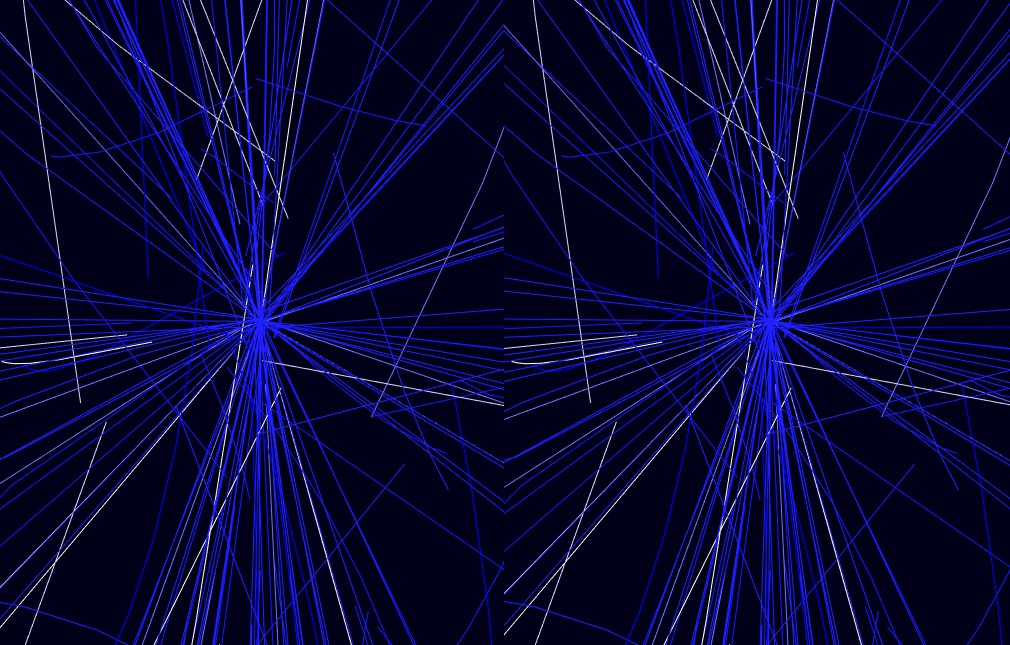
\includegraphics[width=\textwidth]{Stereo_event4047_run226466.jpg}
 		\captionsetup{font={up, footnotesize}}
    	\caption{Dane z pliku event4047\_run226466.json}
 		\label{rys32}
	\end{subfigure}
	\vskip\baselineskip
	\begin{subfigure}{0.90\textwidth}
		\centering
		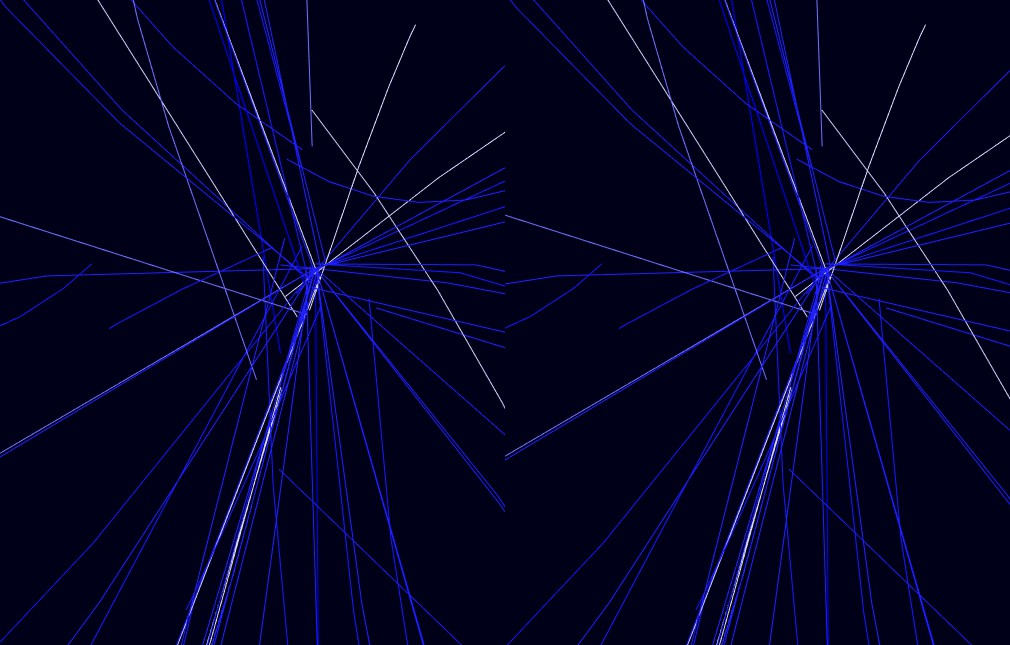
\includegraphics[width=\textwidth]{Stereo_event3055_run226466.jpg}
		\captionsetup{font={up, footnotesize}}
    	\caption{Dane z pliku event3055\_run226466.json}
		\label{rys33}
	\end{subfigure}	

    \label{rys31}
\end{figure}

\newpage
\section{Zawartość płyty CD}
Płyta CD zawiera folder z oprogramowaniem, w tym folderze umieszczone są: 
\begin{itemize}
\itemi Folder Documents zawiera pdf niniejszej pracy.
\itemi Folder Glitter przechowuje potrzebne biblioteki, które przy pierwszym uruchomieniu zostaną zbudowane.
\itemi Folder Headers zawiera wszystkie pliki nagłówkowe programu.
\itemi Folder Shaders gromadzi w jednym miejscu wszystkie moduły cieniujące użyte w programie.
\itemi Folder events.zip przechowuje wszystkie otrzymane pliki JSON z danymi o torach.
\itemi Plik CMakeLists.txt zawiera zestaw instrukcji opisujących pliki wykonywalne, dołączone biblioteki. 
\itemi Plik detector.dae przechowuje model detektora ALICE.
\itemi Plik main.cpp uruchamia program.
\itemi Track.json to plik z danymi o torach cząstki.
\itemi Readme przechowuje instrukcję uruchomienia programu na różnych platformach.
\end{itemize}
\end{appendices}

\newpage
\bibliographystyle{plain} % bibliography style
\bibliography{bibliography} % add bibliography

\newpage
\listoffigures

\newpage
\listoftables

%\newpage
%\listofappendix


\end{document}
